\documentclass[11pt,a4paper,DIV=12]{scrartcl}
\usepackage{scrlayer-scrpage}
\usepackage[utf8]{inputenc}
\usepackage{fouriernc}
\usepackage[T1]{fontenc}
\usepackage[english]{babel}
\usepackage[hidelinks]{hyperref}
\usepackage{natbib}
\usepackage{url}
\usepackage{amsmath}
\usepackage{amsfonts}
\usepackage{amssymb}
\usepackage{trfsigns}
\usepackage{marvosym}
\usepackage{nicefrac}
\usepackage{enumitem}
\usepackage{graphicx}
\usepackage{subcaption}
%\usepackage{subfig}
\usepackage{xcolor}
\usepackage{comment}
\usepackage{framed}
\usepackage{tikz}
%\usepackage{circuitikz}
%\usepackage{pgfplots}
\usepackage{bm}

%matplotlib colors:
\definecolor{C0}{HTML}{1f77b4}
\definecolor{C1}{HTML}{ff7f0e}
\definecolor{C2}{HTML}{2ca02c}
\definecolor{C3}{HTML}{d62728}
\definecolor{C7}{HTML}{7f7f7f}

\newcommand{\mydft}{\mbox{\setlength{\unitlength}{0.1em}%
                            \begin{picture}(20,10)%
                              \put(2,3){\circle{4}}%
                              \put(4,3){\line(1,0){4.75}}%
                              \multiput(8.625,3.15)(0.25,0.25){11}{%
                                \makebox(0,0){\rmfamily\tiny .}}%
                              \put(17,3){\line(-1,0){5.75}}%
                              %\put(18,3){\circle*{4}}%
                              \put(6,-4){\scriptsize $N$}
                            \end{picture}%
                           }
                      }

\newcommand{\myDFT}{\mbox{\setlength{\unitlength}{0.1em}%
                            \begin{picture}(20,10)%
                              %\put(2,3){\circle*{4}}%
                              \put(3,3){\line(1,0){5.75}}%
                              \multiput(11.375,3.15)(-0.25,0.25){11}{%
                                \makebox(0,0){\rmfamily\tiny .}}%
                              \put(16,3){\line(-1,0){4.75}}%
                              \put(18,3){\circle{4}}%
                              \put(6,-4){\scriptsize $N$}
                            \end{picture}%
                           }
                      }

\bibliographystyle{abbrvnat}
\newcommand{\red}{\textcolor{red}}
\specialcomment{Loesung}{\begin{framed}\noindent}{\end{framed}\noindent}
%\excludecomment{Loesung}


\begin{document}
{\raggedleft Sascha Spors\\
Professorship Signal Theory and Digital Signal Processing\\
Institute of Communications Engineering (INT)\\
Faculty of Computer Science and Electrical Engineering (IEF)\\
University of Rostock, Germany\\}
\vspace{0.5cm}
\noindent This tutorial is provided as Open Educational Resource (OER),
to be found at\\
\url{https://github.com/spatialaudio/digital-signal-processing-exercises}\\
accompanying the DSP lecture\\
\url{https://github.com/spatialaudio/digital-signal-processing-lecture}\\
Both OERs are licensed under i) the Creative Commons Attribution 4.0 International
License for text and graphics and ii) under the MIT License for software.
%
Please attribute this special work as
\textit{Frank Schultz, Digital Signal Processing - A
Tutorial Featuring Computational Examples, Spectral Analysis of Deterministic,
Discrete-Time Signals} with the github URL.
\newline

\textbf{Digital Signal Processing Tutorial 1 \& 2, Winter Semester 2020/21}
(Course \#24505)\\
authors: Frank Schultz (concept, initial draft, OER version),
Vera Erbes (proof read, validation, translation from German to English), https://github.com/robhau
(Matlab to Python porting for graphics code)\\
Feel free to contact frank.schultz@uni-rostock.de

%------------------------------------------------------------------------------
\section*{\underline{Spectral Analysis of Deterministic, Discrete-Time Signals}}
\renewcommand{\contentsname}{}
\tableofcontents
\vspace{.7cm}

%\clearpage
\section{Discrete Fourier Transform (DFT)}
Why just another DFT tutorial? Well, this is a collection of calculus,
graphs and exercises that the authors found useful for teaching purposes
and which evolved over the last decade.
%
The didactical approach follows \cite{Rabiner1975}, \cite{Kammeyer2002},
\cite{Moeser2011}.
%
Furthermore, a compact link to linear algebra fundamentals seems to be
reasonable, since (statistical) signal processing, such as machine learning,
heavily relies on matrix algebra. For that, \cite{Strang2019} is a brilliant
resource.

% ---------------------------------------------------------------------------------
\subsection{DFT Definition Conventions}
The discrete Fourier transform (DFT, often interpreted as the signal analysis
stage) and
its counterpart, i.e. the inverse DFT (IDFT, often interpreted as the signal
synthesis stage)
are defined as
\begin{framed}
%
\begin{equation}
X[\mu]=\sum_{k=0}^{N-1}x[k]\cdot W_N^{-k\mu} \hspace{2cm}
x[k]=\frac{1}{N}\sum_{\mu=0}^{N-1}X[\mu]\cdot W_N^{+k\mu}
\end{equation}
using the so-called twiddle factor or DFT kernel
\begin{equation}
W_N=\e^{+\im\frac{2\pi}{N}}
\end{equation}
%
relating an $N$ samples discrete-time signal $x[k]$ and its $N$ coefficients
(also called DFT bins) discrete-frequency DFT spectrum $X[\mu]$.
%
We might use the operator notation
\begin{align}
\text{DFT: }x[k] &\quad\mydft\quad X[\mu]\\
\text{IDFT: }X[\mu] &\quad\myDFT\quad x[k].
\end{align}
%
\end{framed}
%
In general, the DFT/IDFT supports $x[k]\in \mathbb{C}$ and
$X[\mu]\in \mathbb{C}$.
%
Later, some useful relations will be obtained when assuming
$x[k]\in\mathbb{R}$.
%
In the literature, the DFT pair may be differently defined, such as e.g.
\begin{align}
&X[\mu]=\underbrace{{\frac{1}{N}}}_{K_\text{DFT}}\sum_{n=0}^{N-1}x[k]\cdot W_N^{-k\mu}
\hspace{1cm}\mydft\hspace{1cm}
x[k]=\underbrace{{1}}_{K_\text{IDFT}}\sum_{\mu=0}^{N-1}X[\mu]\cdot W_N^{+k\mu}\\
&X[\mu]=\underbrace{{\frac{1}{\sqrt{N}}}}_{K_\text{DFT}}\sum_{n=0}^{N-1}x[k]\cdot W_N^{-k\mu}
\hspace{1cm}\myDFT\hspace{1cm}
x[k]=\underbrace{{\frac{1}{\sqrt{N}}}}_{K_\text{IDFT}}\sum_{\mu=0}^{N-1}X[\mu]\cdot W_N^{+k\mu},
\label{eq:orthonorm}
\end{align}
where different normalisation schemes of the sum are applied.
%
In any case a valid DFT pair must fulfill
\begin{align}
K=K_{\text{IDFT}}\cdot K_{\text{DFT}}=\frac{1}{N},
\end{align}
such that
\begin{align}
x[k]&=\text{IDFT}_N\left\{\text{DFT}_N\left\{x[k]\right\}\right\}
\label{eq:x_idft_dft_x}
\\
X[\mu]&=\text{DFT}_N\left\{\text{IDFT}_N\left\{X[\mu]\right\}\right\}.
\label{eq:X_dft_idft_X}
\end{align}
%
Hence, either the factor $K_{\text{IDFT}}$ or the factor $K_{\text{DFT}}$
can be chosen according to
the specific application and then the other parameter is determined due to
$K=\frac{1}{N}$.
%
Another convention is related to the sign of the exp() function in the twiddle
factor:
%
this may also be defined as, cf. \cite{Oppenheim2010},
\begin{equation}
W_N=\e^{-\im\frac{2\pi}{N}}
\end{equation}
if required for specific applications, so we should pay attention to this tiny detail.
%
Note that the DFT/IDFT equations do not care about signal interpretation, they
just transform a vector/signal to another vector/signal;
proper interpretation is up to the user.
%
The general definition of the DFT pair may thus given as
\begin{equation}
X[\mu]=K_\text{DFT}\sum_{k=0}^{N-1}x[k]\cdot W_N^{\mp k\mu}
\hspace{2cm}
x[k]=K_\text{IDFT}\sum_{\mu=0}^{N-1}X[\mu]\cdot W_N^{\pm k\mu}
\end{equation}
using
\begin{equation}
W_N=(\e^{+\im\frac{2\pi}{N}}),
\hspace{1cm}
K_\text{IDFT}\cdot K_\text{DFT}=\frac{1}{N}.
\end{equation}
%
\begin{framed}
%
Fortunately, the majority of DSP-related books and software packages consistently
define the DFT pair with the following conventions
\begin{align}
X[\mu] = \mathrm{DFT}_N\{x[k]\} = &\sum_{k=0}^{N-1} x[k] \, (\e^{-\im\frac{2\pi}{N}})^{k \cdot \mu}
\hspace{0.5cm}
\text{numpy: \texttt{X=np.fft.fft(x)}, Matlab: \texttt{X=fft(x)}}
\label{eq:DFT}\\
x[k] = \mathrm{IDFT}_N\{X[\mu]\} = \frac{1}{N} &\sum_{\mu=0}^{N-1} X[\mu] \, (\e^{+\im\frac{2\pi}{N}})^{k \cdot \mu}
\hspace{0.4cm}
\text{numpy: \texttt{x=np.fft.ifft(X)}, Matlab: \texttt{x=ifft(X)}}
\label{eq:IDFT}
\end{align}
which will also be used throughout the DSP lecture and tutorial.
%
\end{framed}
%
This convention implies that positive constant group delays in the DFT spectrum
$X$ are interpreted as causal signal delays for $x$.

\subsection{Discrete-Time Fourier Transform (DTFT)}
The DTFT pair using the continuous discrete-time
frequency variable $\Omega$
\begin{align}
X(\Omega)=&\sum_{k=-\infty}^\infty x[k]\,\e^{-\im\Omega k}
\label{eq:DTFT}\\
x[k]=\frac{1}{2\pi}&\int\limits_{-\pi}^\pi X(\Omega)\,\e^{+\im\Omega k}\text{d}\Omega
\end{align}
is defined with the same signs in the exp() function
and the prefactor $\frac{1}{2\pi}$
belonging to the synthesis equation in the same way as for the used definition
of the DFT pair.

% -----------------------------------------------------------------------------
\subsection{Link to Linear Algebra}
The DFT is basically a fundamental linear algebra problem, i.e.
solving a set of linear equations, or in another train of thought: transferring
one vector to another vector in hope for more convenient data representation,
such as here either for spectrum analysis or signal synthesis.
%
Of course it is not pure hope which helps us performing these tasks, but
a very appropriate and intended choice of a vector base that solves our problem.
%
This vector base is probably one of the most beautiful in linear algebra,
in any case it is one the most important ones.
%
Therefore, it is worth to grasp these linear algebra links for an in-depth
understanding of the DFT.
%
\cite{Strang2019} is highly recommended lecture for further reading.

\subsubsection{Roots on the Unit Circle}

The DFT of length $N$ is an excellent example using a special
base of orthogonal vectors whose entries are set up from the roots of the $z^N=1$
equation, i.e. equiangularly distributed locations along the unit circle
within the complex $z$-plane, cf. Fig.~\ref{fig:DFT_UnitCircle}.
%
\begin{figure}[b]
\center
\begin{tikzpicture}[scale=1.5]
\def \tic {0.05}
%
\begin{scope}
\draw[C3, thick] (0,0) circle(1);  % unit circle, i.e. DTFT domain
\draw[C3] (0.78,-0.78) node[right]{DTFT $z=\e^{\im\Omega}$};
\draw[C0] (0.78,-1.15) node[right]{DFT $z_\mu = \e^{\im\frac{2\pi}{4}\mu}$};
%
\draw (1+2*\tic,-3*\tic) node{$1$}; % indicate that this is the unit circle
\draw[->] (-1.25,0)--(1.75,0) node[right]{$\Re\{z\}$}; % axis label
\draw[->] (0,-1.25)--(0,1.5) node[above]{$\Im\{z\}$}; % axis label
%
\draw[C0, ultra thick] (0,+1) node{\Huge $\circ$};
\draw[C0, ultra thick] (0,-1) node{\Huge $\circ$};
\draw[C0, ultra thick] (+1,0) node{\Huge $\circ$};
\draw[C0, ultra thick] (-1,0) node{\Huge $\circ$};
%
\draw[] (+1+1*\tic,4*\tic) node[right]{$z_0=1$};
\draw[] (2*\tic,+1+4*\tic) node[right]{$z_1=W_4=\e^{\im\frac{2\pi}{4}}$};
\draw[] (-1+4*\tic,4*\tic) node{$z_2$};
\draw[] (4*\tic,-1+4*\tic) node{$z_3$};
%
\draw[->] (0.25,0) node[above]{$\frac{2\pi}{4}$} arc (0:90:0.25) ;
%
\draw[] (0,2.25) node{Solutions for $z^4 = 1$, $N=4$ DFT};
\end{scope}
%
\begin{scope}[xshift=5cm]
\draw[C3, thick] (0,0) circle(1);  % unit circle, i.e. DTFT domain
\draw[C3] (0.78,-0.78) node[right]{DTFT $z=\e^{\im\Omega}$};
\draw[C0] (0.78,-1.15) node[right]{DFT $z_\mu = \e^{\im\frac{2\pi}{5}\mu}$};
%
\draw (1+2*\tic,-3*\tic) node{$1$}; % indicate that this is the unit circle
\draw[->] (-1.25,0)--(1.75,0) node[right]{$\Re\{z\}$}; % axis label
\draw[->] (0,-1.25)--(0,1.5) node[above]{$\Im\{z\}$}; % axis label
%
\draw[white] (0,-1)--(0,+1);
\draw[white] (-1,0)--(+1,0);
%
\draw[C0, ultra thick] (1,0) node{\Huge $\circ$};
\draw[C0, ultra thick] (0.30902, 0.95106) node{\Huge $\circ$};
\draw[C0, ultra thick] (-0.80902, 0.58779) node{\Huge $\circ$};
\draw[C0, ultra thick] (-0.80902,- 0.58779) node{\Huge $\circ$};
\draw[C0, ultra thick] (0.30902,- 0.95106) node{\Huge $\circ$};
%
\draw[] (+1+1*\tic,4*\tic) node[right]{$z_0=1$};
\draw[] (0.30902+1*\tic, 0.95106+3*\tic) node[right]{$z_1=W_5=\e^{\im\frac{2\pi}{5}}$};
\draw[] (-0.80902-4*\tic, 0.58779+4*\tic) node{$z_2$};
\draw[] (-0.80902-4*\tic,- 0.58779-4*\tic) node{$z_3$};
\draw[] (0.30902+4*\tic,- 0.95106-4*\tic) node{$z_4$};
%
\draw[-] (0,0) -- (1,0);
\draw[-] (0,0) -- (0.30902, 0.95106);
\draw[-] (0,0) -- (-0.80902, 0.58779);
\draw[-] (0,0) -- (-0.80902,- 0.58779);
\draw[-] (0,0) -- (0.30902,- 0.95106);
\draw[->] (0.25,0) node[above]{$\frac{2\pi}{5}$} arc (0:72:0.25) ;
%
\draw[] (0,2.25) node{Solutions for $z^5 = 1$, $N=5$ DFT};
\end{scope}
%
\end{tikzpicture}
\caption{DFT frequencies (blue dots) on the unit circle (red) in the complex $z$-plane.}
\label{fig:DFT_UnitCircle}
\end{figure}
%
For a complete DFT or IDFT, cf. \eqref{eq:DFT}, \eqref{eq:IDFT}, all
pairs $k \cdot \mu$ are required.
%
It is useful to create an $N \times N$ matrix from an outer product as
%
\begin{align}
\bm{K} &=
\begin{bmatrix}
0\\
1\\
2\\
3\\
\vdots\\
N-1
\end{bmatrix}
\cdot
\begin{bmatrix}
0 & 1 & 2 & 3 &\cdots & N-1
\end{bmatrix}\\
&=k \downarrow
\substack{\rightarrow \mu\\
\begin{bmatrix}
0 \cdot 0 & 0 \cdot 1 & 0 \cdot 2 & 0 \cdot 3 & \dots & 0 \cdot (N-1)\\
1 \cdot 0 & 1 \cdot 1 & 1 \cdot 2 & 1 \cdot 3 & \dots & 1 \cdot (N-1)\\
2 \cdot 0 & 2 \cdot 1 & 2 \cdot 2 & 2 \cdot 3 & \dots & 2 \cdot (N-1)\\
3 \cdot 0 & 3 \cdot 1 & 3 \cdot 2 & 3 \cdot 3 & \dots & 3 \cdot (N-1)\\
\vdots & \vdots & \vdots & \vdots & \ddots & \vdots\\
(N-1) \cdot 0 & (N-1) \cdot 1 & (N-1) \cdot 2 & (N-1) \cdot 3 & \dots &  (N-1) \cdot (N-1)
\end{bmatrix}
},
\end{align}
i.e. varying the time index from top to bottom and increasing the
DFT frequency from left to right.
%
The complex number $z_1 = W_N = \e^{+\im\frac{2\pi}{N}}$
from Fig.~\ref{fig:DFT_UnitCircle} is identified as the twiddle factor introduced
beforehand.
%
This corresponds to the special DTFT frequency $\Omega = \frac{2\pi}{N}$.
%
In analogy to the Fourier series, this frequency is the first harmonic for a DFT
of length $N$.
%
The entry $z_0$ obviously corresponds to the frequency $\Omega=0$.
%
The IDFT \eqref{eq:IDFT} precisely requires powers of the twiddle factor forming
the different phasors
$(W_N)^{k\cdot \mu} = (\e^{+\im\frac{2\pi}{N}})^{k\cdot \mu} = \e^{+\im\frac{2\pi}{N} (k\cdot \mu)}$.
%
\subsubsection{Fourier Matrix}
%
That is why matrix $\bm{K}$ was built before: by using element-wise operator $\odot$
%
\begin{equation}
\mathbf{W} =
\e^{+\im\frac{2\pi}{N} \odot \mathbf{K}}
\end{equation}
%
the so called
$N \times N$ Fourier Matrix
%
\begin{align}
\label{eq:FourierMatrix}
\bm{W} =
k \downarrow
\substack{\rightarrow \mu\\
\begin{bmatrix}
\e^{+\im\frac{2\pi}{N} (0 \cdot 0)} & \e^{+\im\frac{2\pi}{N} (0 \cdot 1)} & \e^{+\im\frac{2\pi}{N} (0 \cdot 2)} & \e^{+\im\frac{2\pi}{N} (0 \cdot 3)} & \dots & \e^{+\im\frac{2\pi}{N} (0 \cdot (N-1))}\\
\e^{+\im\frac{2\pi}{N} (1 \cdot 0)} & \e^{+\im\frac{2\pi}{N} (1 \cdot 1)} & \e^{+\im\frac{2\pi}{N} (1 \cdot 2)} & \e^{+\im\frac{2\pi}{N} (1 \cdot 3)} & \dots & \e^{+\im\frac{2\pi}{N} (1 \cdot (N-1))} \\
\e^{+\im\frac{2\pi}{N} (2 \cdot 0)} & \e^{+\im\frac{2\pi}{N} (2 \cdot 1)} & \e^{+\im\frac{2\pi}{N} (2 \cdot 2)} & \e^{+\im\frac{2\pi}{N} (2 \cdot 3)} & \dots & \e^{+\im\frac{2\pi}{N} (2 \cdot (N-1))}\\
\e^{+\im\frac{2\pi}{N} (3 \cdot 0)} & \e^{+\im\frac{2\pi}{N} (3 \cdot 1)} & \e^{+\im\frac{2\pi}{N} (3 \cdot 2)} & \e^{+\im\frac{2\pi}{N} (3 \cdot 3)} & \dots & \e^{+\im\frac{2\pi}{N} (3 \cdot (N-1))}\\
\vdots & \vdots & \vdots & \vdots & \ddots & \vdots\\
\e^{+\im\frac{2\pi}{N} ((N-1) \cdot 0)} & \e^{+\im\frac{2\pi}{N} ((N-1) \cdot 1)} & \e^{+\im\frac{2\pi}{N} ((N-1) \cdot 2)} & \e^{+\im\frac{2\pi}{N} ((N-1) \cdot 3)} & \dots &  \e^{+\im\frac{2\pi}{N} ((N-1) \cdot (N-1))}
\end{bmatrix}
}
\end{align}
is set up.
%
In textbooks the short version is often given using powers of twiddle factor $W_N$
\begin{align}
\bm{W} =
k \downarrow
\substack{\rightarrow \mu\\
\begin{bmatrix}
1 & 1 & 1 & 1 & \dots & 1\\[1em]
1 & W_N^1 & W_N^2 & W_N^3 & \dots & W_N^{(N-1)}\\[1em]
1 & W_N^2 & W_N^4 & W_N^6 & \dots & W_N^{2(N-1)}\\[1em]
1 & W_N^3 & W_N^6 & W_N^9 & \dots & W_N^{3(N-1)}\\[1em]
\vdots & \vdots & \vdots &\vdots &\ddots & \vdots\\[1em]
1 & W_N^{(N-1)} & W_N^{2(N-1)} & W_N^{3(N-1)} & \dots & W_N^{(N-1)(N-1)}
\end{bmatrix}
}.
\end{align}
%
The orthogonal columns---this is the essential idea just like using
orthogonal oscillations in a Fourier series---of the Fourier matrix contain
the samples for complex-valued
oscillations $(\e^{\im \frac{2\pi}{N} k})^\mu$ over time index $k$ for all possible
DFT frequencies $0 \leq \mu \leq N-1$.
%
All these oscillations are $N$-periodic.
%
The first column of $\bm W$ corresponds to $\mu=0$, this column represents a DC discrete-time
signal, i.e. all samples exhibit amplitude one.
%
The second column of $\bm W$ corresponds to $\mu=1$ and contains the $N$ samples of the
first DFT harmonic $x[k|\mu=1]=\e^{+\im \frac{2\pi}{N} k \cdot 1}$,
i.e. one signal period fits exactly into $N$ samples, cf.
Fig.~\ref{fig:dft_eigensignals_columns} top.
%
The third column of $\bm W$ corresponds to $\mu=2$ and contains the $N$ samples of the
second DFT harmonic $x[k|\mu=2]=\e^{+\im \frac{2\pi}{N} k \cdot 2}$,
i.e. two signal periods fit exactly into $N$ samples, cf.
Fig.~\ref{fig:dft_eigensignals_columns} bottom.
%
\begin{figure}[t]
		\centering
		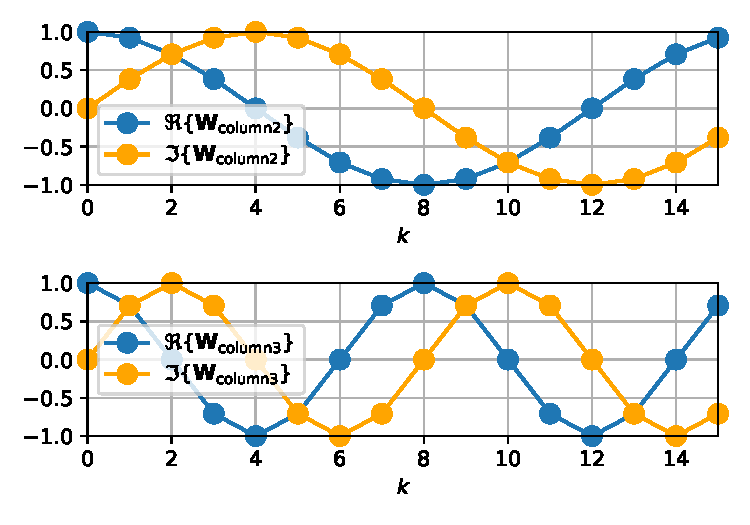
\includegraphics[width=5in, height=3.5in]{graphics/dft_eigensignals_columns.pdf}
		\caption{For the $N=16$ DFT, the complex-valued signals
    $\e^{+ \im \frac{2\pi}{N} k \cdot\mu}$ are shown for $\mu=1$ (top) and for
    $\mu=2$ (bottom).
    These signals correspond to the vectors in the 2nd and 3rd column,
    respectively, of the Fourier matrix $\bm W$.
    We might think of all $N$ signals / column vectors in $\bm W$ as DFT eigensignals
    as these are used for synthesis (IDFT) and analysis (DFT) stages.}
		\label{fig:dft_eigensignals_columns}
\end{figure}



\subsubsection{IDFT as Matrix Operation}
%
Now, let us consider column vectors with $N$ entries
for the discrete-time signal $x[k]$ of length $N$
(actually the signal is periodic in $N$,
the prevailing convention considers the period at time instances
$0 \leq k \leq N-1$)
and its DFT spectrum $X[\mu]$ ($N$-periodic as well,
convention $0\leq \mu \leq N-1$):
%
\begin{align}
\text{discrete-time signal: }
\bm{x}_k =
\begin{bmatrix}
x[k=0]\\
x[k=1]\\
x[k=2]\\
x[k=3]\\
\vdots\\
x[k=N-1]\\
\end{bmatrix}\qquad
\text{DFT spectrum: }
\bm{x}_\mu =
\begin{bmatrix}
X[\mu=0]\\
X[\mu=1]\\
X[\mu=2]\\
X[\mu=3]\\
\vdots\\
X[\mu=N-1]\\
\end{bmatrix}.
\end{align}
%
The IDFT can then be written as matrix multiplication as follows
%
\begin{align}
\label{eq:IDFT_as_Matrix}
\bm{x}_k = \frac{1}{N} \bm{W} \cdot \bm{x}_\mu .
\end{align}
%
The linear combination of the column vectors in $\bm{W}$ weighted by the DFT
spectrum's coefficients $X[\cdot]$ and normalisation by $\nicefrac{1}{N}$
reveals the discrete-time signal synthesis stage
\label{LinComb_for_IDFT}
%
\begin{align*}
\begin{bmatrix}
x[0]\\[1em]
x[1]\\[1em]
x[2]\\[1em]
x[3]\\[1em]
\dots\\[1em]
x[N-1]
\end{bmatrix}
=
\frac{X[0]}{N}
\begin{bmatrix}
1\\[1em]
1\\[1em]
1\\[1em]
1\\[1em]
\dots\\[1em]
1
\end{bmatrix}
+\frac{X[1]}{N}
\begin{bmatrix}
1\\[1em]
W_N^1\\[1em]
W_N^2\\[1em]
W_N^3\\[1em]
\dots\\[1em]
W_N^{(N-1)}
\end{bmatrix}
+\frac{X[2]}{N}
\begin{bmatrix}
1\\[1em]
W_N^2\\[1em]
W_N^4\\[1em]
W_N^6\\[1em]
\dots\\[1em]
W_N^{2(N-1)}
\end{bmatrix}
+\frac{X[3]}{N}
\begin{bmatrix}
1\\[1em]
W_N^3\\[1em]
W_N^6\\[1em]
W_N^9\\[1em]
\dots\\[1em]
W_N^{3(N-1)}
\end{bmatrix}
+
\dots
+\frac{X[N-1]}{N}
\begin{bmatrix}
1\\[1em]
W_N^{1(N-1)}\\[1em]
W_N^{2(N-1)}\\[1em]
W_N^{3(N-1)}\\[1em]
\dots\\[1em]
W_N^{(N-1)(N-1)}
\end{bmatrix}.
\end{align*}
%
It is very similar to Fourier series synthesis: a weigthed superposition of
harmonics and a DC signal.
%
The difference to the Fourier series is, that the DFT exhibits an
$N$-periodic, discrete spectrum of Fourier coefficients,
which induces an $N$-periodic \textbf{and} discrete-time signal.
%
\subsubsection{DFT as Matrix Operation}
\label{Ch:DFTasMatrixOperation}
%
The column vectors $\bm{w}_i$ and $\bm{w}_j$ from matrix $\bm{W}$ (that are
considered for the superposition above) exhibit orthogonality,
i.e. the inner product for complex vectors yields
\begin{align}
\bm{w}_{\text{column i}}^\text{H} \cdot \bm{w}_\text{column j} =
\begin{cases}
N & i=j\\
0 & \text{else}
\end{cases}
\end{align}
using the conjugate transpose operator $(\cdot)^\text{H}$.
%
Again this is very similar to the Fourier series fundamentals, where the
continuous-time signals
$\sin(\mu \omega_0 t)$, $\cos(\mu \omega_0 t)$ and $\e^{\im \mu \omega_0 t}$
are orthogonal to each other for different $\mu\in\mathbb{Z}$.
%

The analysis stage for the discrete-time signal domain, i.e. the DFT
can now be reinvented by some intuition:
How 'much' of the reference signal $\bm{w}_{\text{column i}}$
(any column in $\bm{W}$)
is contained in the discrete-time signal $\bm{x}_k$ that is to be analysed.
%
In signal processing / statistic terms we look for the amount of correlation
of the signals
$\bm{w}_{\text{column i}}$ and $\bm{x}_k$.
%
In linear algebra terms we are interested in the projection\footnote{
A projection in the strict sense of linear algebra would only be obtained
if $\bm{w}_{\text{column i}}$
is a unit vector, which can be easily obtained when normalising by
$\frac{1}{\sqrt{N}}$. See the comment on the unitary matrix property
on pg.~\pageref{pg:unitary}.}
of $\bm{x}_k$ onto
$\bm{w}_{\text{column i}}$, because the length of the resulting projection vector
reveals the amount of correlation, which is precisely one DFT coefficient $X[\cdot]$.
%
The complex inner products $\bm{w}_{\text{column i}}^\text{H} \cdot \bm{x}_k$
reveals these searched quantities.
%
Doing this for all columns of matrix $\bm W$, all DFT coefficients are obtained
(\textbf{vector projection mindset}):
\begin{align}
X[\mu=0] =& \bm{w}_{\text{column 1}}^\text{H} \cdot \bm{x}_k\\
X[\mu=1] =& \bm{w}_{\text{column 2}}^\text{H} \cdot \bm{x}_k\\
X[\mu=2] =& \bm{w}_{\text{column 3}}^\text{H} \cdot \bm{x}_k\\
X[\mu=3] =& \bm{w}_{\text{column 4}}^\text{H} \cdot \bm{x}_k\\
&\vdots\\
X[\mu=N-1] =& \bm{w}_{\text{column N}}^\text{H} \cdot \bm{x}_k.
\end{align}
%
Naturally, all operations can be merged to one single
matrix multiplication using the conjugate transpose of $\bm W$
%
\begin{align}
\bm{W}^\text{H} =
\mu \downarrow
\substack{\rightarrow k\\
\begin{bmatrix}
1 & 1 & 1 & 1 & \dots & 1\\[1em]
1 & W_N^{-1} & W_N^{-2} & W_N^{-3} & \dots & W_N^{-(N-1)}\\[1em]
1 & W_N^{-2} & W_N^{-4} & W_N^{-6} & \dots & W_N^{-2(N-1)}\\[1em]
1 & W_N^{-3} & W_N^{-6} & W_N^{-9} & \dots & W_N^{-3(N-1)}\\[1em]
\vdots & \vdots & \vdots &\vdots &\ddots & \vdots\\[1em]
1 & W_N^{-(N-1)} & W_N^{-2(N-1)} & W_N^{-3(N-1)} & \dots & W_N^{-(N-1)(N-1)}
\end{bmatrix}
}.
\end{align}
%
The DFT is then given as
\begin{align}
\label{eq:DFT_as_Matrix}
\bm{x}_\mu = \bm{W}^\text{H} \cdot \bm{x}_k
\end{align}
yielding the DFT coefficients / spectrum stored in $\bm{x}_\mu$.
%
Here, for the matrix-vector multiplication, a matrix row $\times$ a column vector
is a good mindset to grasp the concept of correlation / projection.
%
The required complex inner product is ensured by taking the conjugate transpose
'beforehand'.


\subsubsection{Fourier Matrix Characteristics}
%
The intuition that led to the DFT as matrix operation is for good reason;
of course there is a strict mathematical proof, which we don't need here.
%
Rather, it is of high importance, that
the matrix $\bm W$ has exceptional characteristics,
cf.~\cite[Ch.~IV.2]{Strang2019}\footnote{
also see Ch.~11 in Frank Schultz, Continuous- and Discrete-Time
Signals and Systems---A Tutorial with Computational Examples,
University of Rostock,
\url{https://github.com/spatialaudio/signals-and-systems-exercises}
}.
%
Generally, for a transform pair we should expect solving a forward and an
inverse problem for two $N \times 1$ vectors $\bm v_1$ and $\bm v_2$,
such as for the set
of equations (\textbf{solving a set of linear equations mindset})
\begin{align}
\bm v_1 = \bm M \bm v_2\qquad \bm v_2 = \bm M^{-1} \bm v_1,
\end{align}
which holds if matrix $\bm M$ is square and has full rank, i.e. it is invertible.
%
For the Fourier matrix the relations
\begin{equation}
\mathbf{W}^{-1}
= \frac{\mathbf{W}^\mathrm{H}}{N}
= \frac{\mathbf{W}^\mathrm{*}}{N}
\end{equation}
hold; $(\cdot)^\mathrm{H}$ is conjugate transpose, $(\cdot)^*$ is
complex conjugate.
%
Inserting this into the DFT equation \eqref{eq:DFT_as_Matrix} reveals the
inverse problem (which is here the analysis stage by our chosen sign convention
in the twiddle factor)
\begin{align}
\bm{x}_\mu = N \bm{W}^{-1} \, \bm{x}_k
\end{align}
and inserting the IDFT equation \eqref{eq:IDFT_as_Matrix} (our forward problem)
into it, yields equality, cf. \eqref{eq:X_dft_idft_X},
\begin{align}
\bm{x}_\mu = N \bm{W}^{-1} \, (\frac{1}{N} \bm{W} \, \bm{x}_\mu) =
\bm x_\mu
\end{align}
as expected.
%
The above relations
$\mathbf{W}^{-1}
= \frac{1}{N} \mathbf{W}^\mathrm{H}
= \frac{1}{N} \mathbf{W}^\mathrm{*}$
are given since $\mathbf{W}$ is a special square, complex
valued and in fact symmetric matrix.
%
Furthermore, recall from above that the normalisation factors can be assigned
differently.
%
\label{pg:unitary}
If the matrix is normalised as $\nicefrac{\bm W}{\sqrt{N}}$, the property
\begin{equation}
\left(\frac{\mathbf{W}}{\sqrt{N}}\right)^\mathrm{H} \, \left(\frac{\mathbf{W}}{\sqrt{N}}\right) = \mathbf{I}
=
\left(\frac{\mathbf{W}}{\sqrt{N}} \right)^{-1} \, \left(\frac{\mathbf{W}}{\sqrt{N}} \right)
\end{equation}
holds, i.e. the complex conjugate transpose is equal to the inverse
$\left(\frac{\mathbf{W}}{\sqrt{N}}\right)^\mathrm{H} =
\left(\frac{\mathbf{W}}{\sqrt{N}} \right)^{-1}$
and due to the matrix symmetry also
$\left(\frac{\mathbf{W}}{\sqrt{N}}\right)^* =
\left(\frac{\mathbf{W}}{\sqrt{N}} \right)^{-1}$
is valid.
%
As a generalisation for complex valued matrices, this implies \textbf{orthonormality
of the so called unitary matrix} $\nicefrac{\bm W}{\sqrt{N}}$.
%
This is the key feature of the Fourier matrix and builds the fundamental of the
DFT:
%
the unitary Fourier matrix spans an orthonormal vector space that is specially
related to the roots of $z^N=1$.
%
\begin{framed}
After all, the DFT pair, this is
\eqref{eq:DFT_as_Matrix} / \eqref{eq:DFT} and
\eqref{eq:IDFT_as_Matrix} / \eqref{eq:IDFT},
is given as
\begin{align}
\text{ DFT: }\bm{x}_\mu = \bm{W}^* \bm{x}_k\qquad
\text{IDFT: }\bm{x}_k = \frac{1}{N} \bm{W} \bm{x}_\mu
\end{align}
using the Fourier Matrix \eqref{eq:FourierMatrix}.
No matrix inversion and transpose, but only complex conjugate operation is
required for the DFT stage.
\end{framed}
%
It is worth to verify that the following DFT pairs with $N=4$ hold with the
chosen conventions
\begin{itemize}
  \item the signal vector $\mathbf{x}_k=[1,1,1,1]^\mathrm{T}$ (pure DC component)
  yields the DFT spectrum $\mathbf{x}_\mu = [4,0,0,0]^\mathrm{T}$
  (energy only at 'zero'-th frequency bin, i.e. DC)
  \item the DFT spectrum $\mathbf{x}_\mu = [1,1,1,1]^\mathrm{T}$
  (all frequencies exhibit equal energy) yields $\mathbf{x}_k = [1,0,0,0]^\mathrm{T}$
  (the discrete Dirac impulse)
\end{itemize}

%------------------------------------------------------------------------------
\subsection{FFT as a Fast Calculation of the DFT}
%
A straightforward implementation of the DFT/IDFT equations directly or
by its matrix versions demands very high computing load for large $N$ and
is prone to numerical precision errors.
%
Fortunately, the computing load can be considerably reduced by saving many
redundant calculations, which at the same time reduces numerical errors.
%

For example, most obviously the same $W_N^{k\mu}$ is derived for $\mu=1$, $k=2$
and $\mu=2$, $k=1$, cf. the entries of the matrices $\mathbf{K}$ and $\mathbf{W}$.
%
For large $N$, many angles $\frac{2\pi}{N}k\mu$ are equivalent.
%
This is exemplarily shown in Fig.~\ref{Twiddle1}, Fig.~\ref{Twiddle2} and
Fig.~\ref{Twiddle3} for $N=8$, $N=9$ and $N=48$ DFTs.
%
These plots indicate certain symmetries, which is to be expected since the
underlying matrices exhibit symmetry as well.

Algorithms that make use of these symmetries in order to reduce or simplify
computation steps are subsumed as Fast Fourier Transform (FFT).
%
Explained in a sloppy way, FFTs calculate certain repeatedly used twiddle factor
results only once.
%
An initial FFT algorithm was proposed by \cite{Cooley1965},
that relies on $N=2^m$, $m\in\mathbb{N}$.
%
With a linear algebra driven mindset, FFT is about finding
suitable matrix factorisations of $\bm W$ to avoid the calculation of the full
matrix multiplication.
%
This involves sparse matrices and plain
vector permutations (which not need to be calculated as matrix operations) and
thus reduces multiplications/additions.
%
We will reinvent the basic concept in a homework assignment.
%
Nowadays, many improved FFT algorithms exist, so that if $N$
is accessible for a prime factorisation, an FFT can be calculated with much less
processing load than a DFT.
%
In fact, the invention of fast DFT calculation via FFT algorithms
is a (if not \textit{the}) milestone in DSP allowing for the huge
technological progress over the last decades.



\begin{figure}[b!]
		\centering
		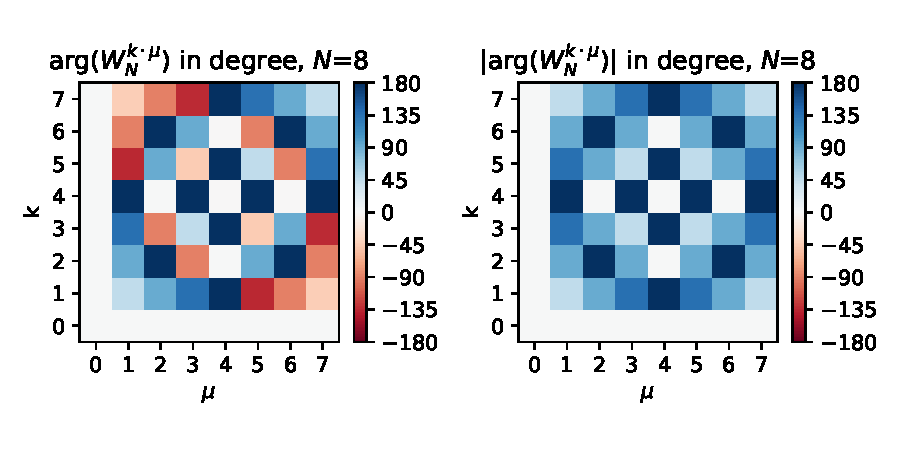
\includegraphics[width=6in, height=3in]{graphics/TwiddleFactorMatrix_N8.pdf}
		\caption{$\text{arg}(W_N^{\mu k})$ (left) and $|\text{arg}(W_N^{\mu k})|$
		(right) as matrix over $\mu$ and $k$ for $N=8$.}
		\label{Twiddle1}
\end{figure}
\begin{figure}[t]
		\centering
		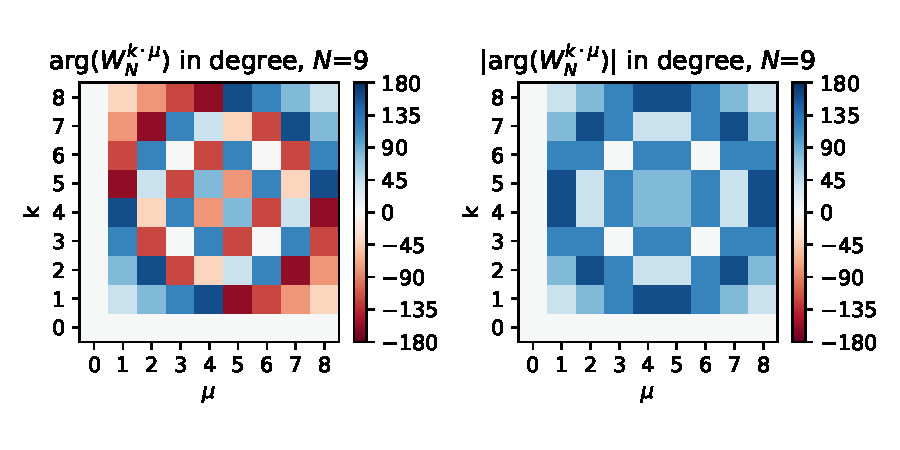
\includegraphics[width=6in, height=3in]{graphics/TwiddleFactorMatrix_N9.pdf}
		\caption{$\text{arg}(W_N^{\mu k})$ (left) and $|\text{arg}(W_N^{\mu k}|$
		(right) as matrix over $\mu$ and $k$ for $N=9$.}
		\label{Twiddle2}
\end{figure}
\begin{figure}
		\centering
		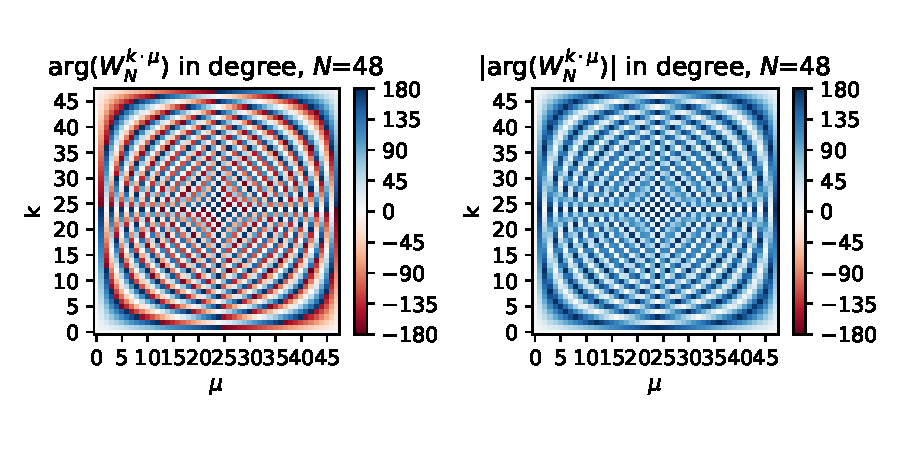
\includegraphics[width=6in, height=3in]{graphics/TwiddleFactorMatrix_N48.pdf}
		\caption{$\text{arg}(W_N^{\mu k})$ (left) and $|\text{arg}(W_N^{\mu k})|$
		(right) as matrix over $\mu$ and $k$ for $N=48$.}
		\label{Twiddle3}
\end{figure}

% ---------------------------------------------------------------------------------
\subsection{DFT Frequency Resolution}
The relation between physical temporal frequency $f$, sampling frequency $f_s$
and discrete-time angular frequency $\Omega$ is known as
\begin{equation}
\Omega=2\pi \frac{f}{f_s}=\frac{\omega}{f_s}.
\end{equation}
%
Furthermore, the twiddle factor and the Fourier matrix tell us that
the unit circle is equiangularly sampled. cf. Fig.~\ref{fig:DFT_UnitCircle}.
%
This means that the angular frequency resolution
\begin{equation}
\Delta \Omega = \frac{2\pi}{N}
\end{equation}
holds.
%
From both equations
\begin{equation}
\Delta \Omega=2\pi \frac{\Delta f}{f_s}=\frac{\Delta \omega}{f_s}\equiv
\Delta \Omega = \frac{2\pi}{N}
\end{equation}
we can deduce the DFT resolution in terms of the physical frequency $f$ as
\begin{equation}
\boxed{\Delta f = \frac{f_s}{N}}.
\end{equation}
%
This corresponds to the frequency distance between two spectral lines, i.e.
between two DFT bins.
%
From that, all so called eigenfrequencies of the DFT, i.e. frequencies where
the DFT bins are located, can be derived as
\begin{equation}
\boxed{f_\text{DFT}=\mu \Delta f=\mu\frac{f_s}{N}
\hspace{5mm}\text{for}\hspace{5mm}
0\leq \mu\leq N-1,\,\,\mu\in\mathbb{N}}.
\end{equation}
%
These DFT eigenfrequencies can also be given for the discrete-time angular
frequency
\begin{equation}
\Omega_\text{DFT} =
\mu \Delta \Omega =
\mu \frac{2\pi}{N} =
\frac{2\pi f_\text{DFT}}{f_s}.
\label{eq:OmegaDFT}
\end{equation}

% -----------------------------------------------------------------------------
\subsection{Periodicity and Symmetry of the DFT}
The signals $x[k]$ and $X[\mu]$ of a DFT pair exhibit a periodicity of $N$.
%
This is shown with $k,\mu,k',m\in\mathbb{Z}$:
\begin{align}
x[k']&=\frac{1}{N}\sum_{\mu=0}^{N-1}X[\mu]\e^{\im\frac{2\pi}{N}k'\mu}\\
x[k'=k+m N]&=\frac{1}{N}\sum_{\mu=0}^{N-1}X[\mu]\e^{\im\frac{2\pi}{N}(k+mN)\mu}\\
&=\frac{1}{N}\sum_{\mu=0}^{N-1}X[\mu]\e^{\im\frac{2\pi}{N}k\mu}\cdot\underbrace{\e^{\im\frac{2\pi}{N}mN\mu}}_{=1}=x[k].
\end{align}
%
A similar proof yields the identity $X[\mu]=X[\mu+mN]$, cf.
Fig.~\ref{Periodicity_DFT}.
%
This is equivalent to a DTFT spectrum that exhibits a $2\pi$ periodicity, i.e.
$X(\Omega)=X(\Omega+m\cdot2\pi)$.
%
The baseband of the DFT for $0\leq\mu\leq N-1$ corresponds to the spectrum of
the signal $x[k]$ for $0\leq k\leq N-1$.
%
Thus, both signals $x[k]$ and $X[\mu]$ inherently exhibit periodicity with $N$.
\begin{figure}[b!]
		\centering
		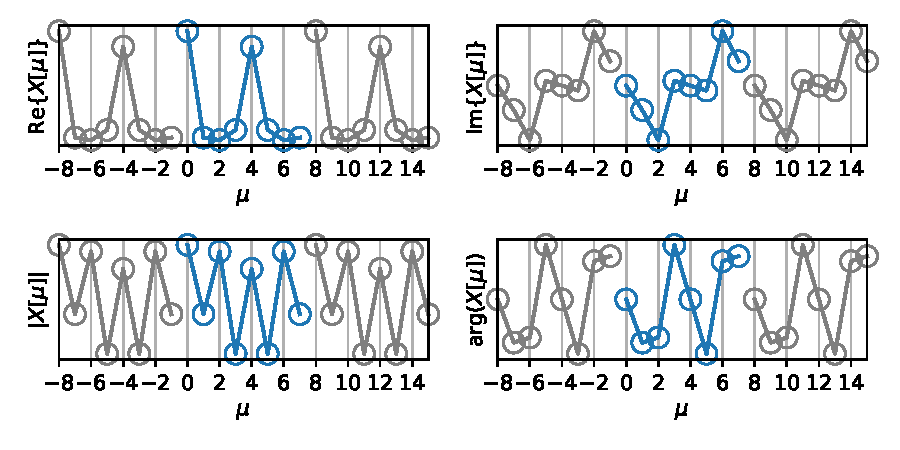
\includegraphics[width=6in, height=3in]{graphics/Periodicity_DFT.pdf}
		\caption{Periodicity of the DFT for a real signal with $N=8$,
		blue: baseband, black: periodic repetitions.}
		\label{Periodicity_DFT}
\end{figure}%

A further very important characteristic of the DFT spectrum is observed,
when $x[k]\in\mathbb{R}$ (such as audio, image and video signals) is assumed.
%
Then the symmetries
\begin{align}
\text{Re}\left\{X\left[\frac{N}{2}+m\right]\right\}&=\text{Re}\left\{X\left[\frac{N}{2}-m\right]\right\}, \hspace{5mm} \text{Im}\left\{X\left[\frac{N}{2}+m\right]\right\}=-\text{Im}\left\{X\left[\frac{N}{2}-m\right]\right\},\\
\left|X\left[\frac{N}{2}+m\right]\right|&=\left|X\left[\frac{N}{2}-m\right]\right|, \hspace{1.3cm} \arg\left(X\left[\frac{N}{2}+m\right]\right)=-\arg\left(X\left[\frac{N}{2}-m\right]\right)
\end{align}
%
hold that can be written shortly as
%
\begin{equation}
X\left[\frac{N}{2}+m\right]=X\left[\frac{N}{2}-m\right]^*,
\label{eq:Symmetry_DFT}
\end{equation}
%
with $()^*$ again denoting complex conjugate operation.
%
Think of $N$ as being an even number here, so $m\in \mathbb{Z}$.
%
The case of odd-numbered $N$ is considered later.
%
The symmetry property of eq.~\eqref{eq:Symmetry_DFT} is shown by inserting and
simplifying
\begin{align}
X\left[\mu=\frac{N}{2}+m\right]&=\sum_{k=0}^{N-1}x[k]\e^{-\im\frac{2\pi}{N}k{\left(\frac{N}{2}+m\right)}}=\sum_{k=0}^{N-1}x[k]\e^{-\im\pi k}\cdot\e^{-\im\frac{2\pi}{N}km},\\
X\left[\mu=\frac{N}{2}-m\right]&=\sum_{k=0}^{N-1}x[k]\e^{-\im\frac{2\pi}{N}k{\left(\frac{N}{2}-m\right)}}=\sum_{k=0}^{N-1}x[k]\e^{-\im\pi k}\cdot\e^{\im\frac{2\pi}{N}km}.
\end{align}
%
The sum of two complex numbers $a,b\in\mathbb{C}$ is just $(a+b)^*=a^*+b^*$.
Recall that $\e^{-\im\pi k}=\pm 1\in\mathbb{R}$.
%
With the assumption $x[k]\in\mathbb{R}$ it can then be proved
\begin{align}
X\left[\mu=\frac{N}{2}-m\right]^*&=\left(\sum_{k=0}^{N-1}x[k]\e^{-\im\pi k}\cdot\e^{\im\frac{2\pi}{N}km}\right)^*\\
&=\sum_{k=0}^{N-1}x[k]\e^{-\im\pi k}\cdot\left(\e^{\im\frac{2\pi}{N}km}\right)^*\\
&=\sum_{k=0}^{N-1}x[k]\e^{-\im\pi k}\e^{-\im\frac{2\pi}{N}km}\\
&=X\left[\mu=\frac{N}{2}+m\right].
\end{align}
%
Since the discrete DFT spectrum is only defined at $\mu\in\mathbb{Z}$
$m$ must be defined as follows
\begin{align}
m=\begin{cases}M&\text{for even }N\\
M+\frac{1}{2}&\text{for odd }N\end{cases}
\end{align}
%
using $M\in\mathbb{Z}$, cf.~Fig.~\ref{Symmetry_DFT_N8} and Fig.~\ref{Symmetry_DFT_N9}.
%
\begin{figure}
		\centering
		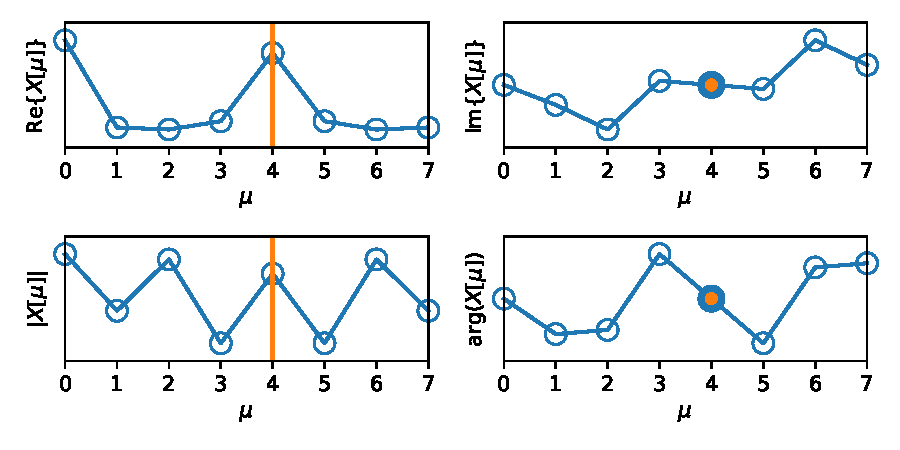
\includegraphics[width=6in, height=3in]{graphics/Symmetry_DFT_N8.pdf}
		\caption{Symmetry of the DFT for $x[k]\in\mathbb{R}$ with $N=8$.
		Point and axis for symmetry is at $\frac{N}{2}=4$.
		Left: real part and magnitude of $X[\mu]$ are axisymmetric,
		right: imaginary part and phase of $X[\mu]$ are point-symmetric.}
		\label{Symmetry_DFT_N8}
\end{figure}
\begin{figure}
		\centering
		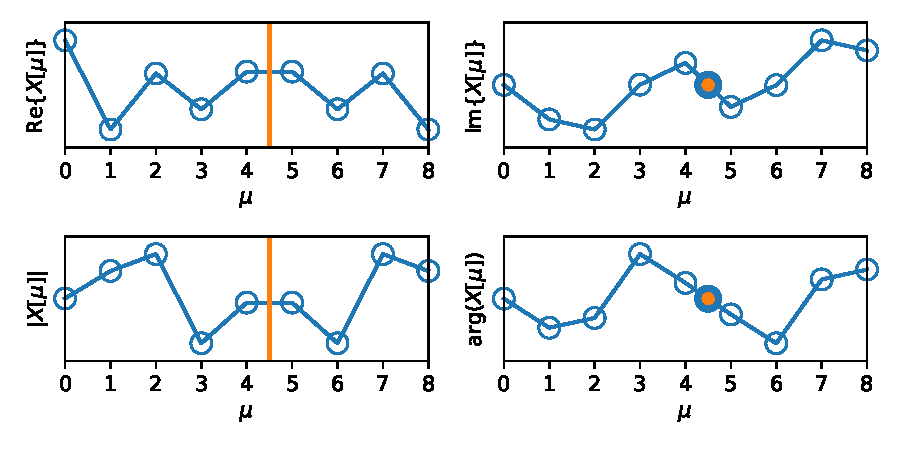
\includegraphics[width=6in, height=3in]{graphics/Symmetry_DFT_N9.pdf}
		\caption{Symmetry of the DFT for $x[k]\in\mathbb{R}$ with $N=9$.
		Point and axis for symmetry is at $\frac{N}{2}=4.5$, i.e. between two DFT bins.
		Left: real part and magnitude of $X[\mu]$ are axisymmetric,
		right: imaginary part and phase of $X[\mu]$ are point-symmetric.}
		\label{Symmetry_DFT_N9}
\end{figure}
%
Due to the periodicity of $X[\mu]$ in general and the special $\frac{N}{2}$
symmetries of $X[\mu]$ when $x[k]\in\mathbb{R}$
(point-symmetric for imaginary part and phase, axisymmetric for real part and
magnitude, cf. again Fig.~\ref{Symmetry_DFT_N8} and Fig.~\ref{Symmetry_DFT_N9})
some information is redundant in the DFT spectrum.
%
For the interpretation of the DFT spectrum, only
\begin{align}
M&=\frac{N}{2}+1 \hspace{5mm}\text{for even }N\nonumber\\
M&=\frac{N+1}{2} \hspace{5mm}\text{for odd }N
\end{align}
bins contain non-redundant information.
%
This corresponds to the frequency band from DC ($f=0$ Hz) to half the sampling
frequency ($f_s/2$).
%
It is defined for \textbf{even} $N$ as
\begin{equation}
0\leq\mu\Delta f\leq\frac{f_s}{2} \hspace{5mm}\text{for}\hspace{5mm} 0\leq\mu\leq\frac{N}{2}
\end{equation}
and for \textbf{odd} $N$ as
\begin{equation}
0\leq\mu\Delta f<\frac{f_s}{2} \hspace{5mm}\text{for}\hspace{5mm} 0\leq\mu\leq\frac{N-1}{2}.
\end{equation}
%
Thus, for even $N$ the symmetry axis $\mu=\frac{N}{2}$ is exactly at the bin
indicating half of the sampling frequency
%
\begin{equation}
f=\mu\frac{f_s}{N}\rightarrow\frac{N}{2}\frac{f_s}{N}=\frac{f_s}{2},
\end{equation}
%
whereas for odd $N$ the symmetry axis is located between the two bins around
$\frac{f_s}{2}$.
%
Therefore, an odd $N$ DFT does not include the 'half of the sampling frequency'
bin, cf.~Fig.~\ref{DFT_Eigenfrequenzen_N4_N5}, Fig.~\ref{DFT_Eigenfrequenzen_N8_N9}.

% -----------------------------------------------------------------------------
\subsection{DFT as Sampling of a DTFT Spectrum}
The following discussion of the discrete Fourier transform (DFT) as a sampled
DTFT and explanations concerning windowing were inspired by the
script \cite{Moeser2011}. A similar didactic concept
is approached in \cite[Ch.~7.3,~7.4]{Kammeyer2002} and \cite{Rabiner1975}.

The DFT contains all possible spectral information that can be derived from the
signal.
%
Since $N$ time samples are available, only maximum $N$ (complex valued) spectral
samples are available; for $x[k]\in\mathbb{R}$ less than $N$ samples contain
non-redundant information as shown above.
%
The DFT can be derived by sampling the DTFT spectrum equiangularly on the unit
circle with $\Delta\Omega=\frac{2\pi}{N}$,
cf.~Fig.~\ref{DFT_Eigenfrequenzen_N4_N5}, Fig.~\ref{DFT_Eigenfrequenzen_N8_N9}.
%
\begin{figure}
		\centering
		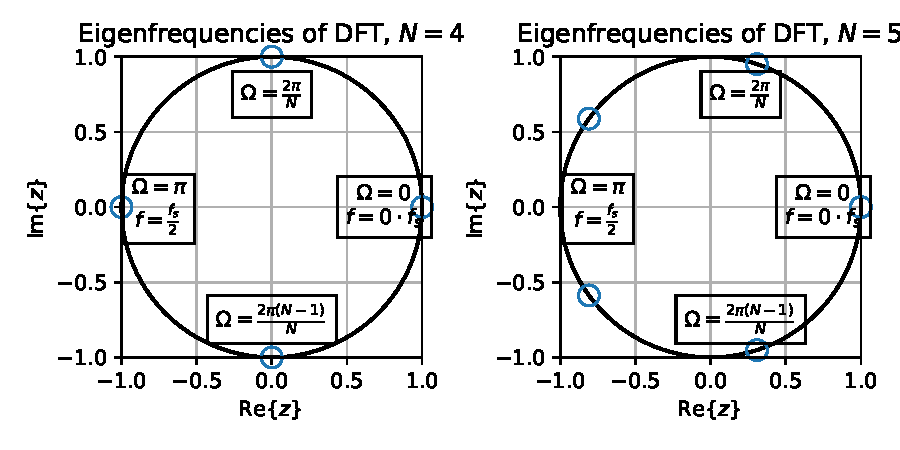
\includegraphics[width=6in, height=3in]{graphics/DFT_Eigenfrequencies_N4_N5.pdf}
		\caption{DFT eigenfrequency locations on the unit circle for $N=4$ (left),
		$N=5$ (right).}
		\label{DFT_Eigenfrequenzen_N4_N5}
\end{figure}
\begin{figure}
		\centering
		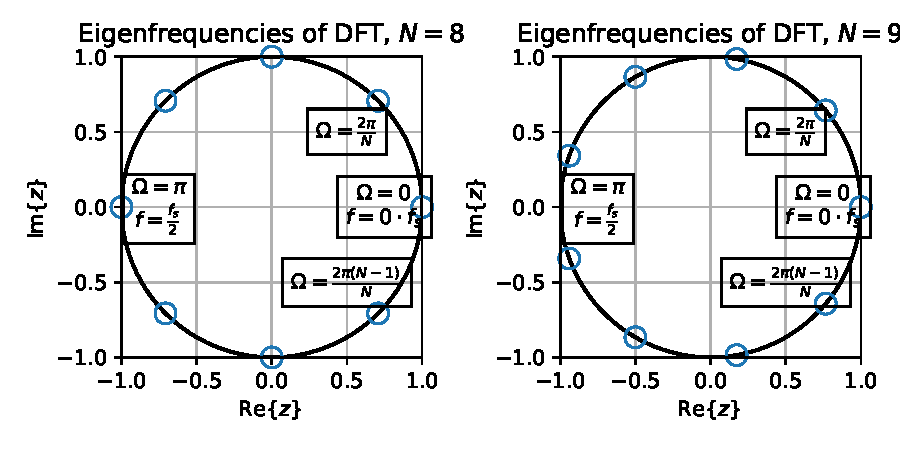
\includegraphics[width=6in, height=3in]{graphics/DFT_Eigenfrequencies_N8_N9.pdf}
		\caption{DFT eigenfrequency locations on the unit circle for $N=8$ (left),
		$N=9$ (right).}
		\label{DFT_Eigenfrequenzen_N8_N9}
\end{figure}
%
Thinking of the DFT $X[\mu]$ as being the spectrum of the non-zero part of a
sampled one-time signal $x[k]$ for $0\leq k\leq N-1$, $x[k]=0$ for all other
$k$ (so-called \textit{single signal model} \cite{Moeser2011}), inversely allows
for interpolation towards the DTFT spectrum.
%
To this end, the synthesis equation for the one-time signal eq.~\eqref{eq:IDFT}
%
\begin{equation}
x[k]=\frac{1}{N}\cdot\sum_{\mu=0}^{N-1}X[\mu]\cdot\e^{\im\frac{2\pi}{N}k\mu}
\end{equation}
%
is inserted into the analysis equation of the DTFT eq.~\eqref{eq:DTFT} and gets
rearranged:
\begin{align}
X(\Omega)&=\sum_{k=-\infty}^\infty x[k]\cdot\e^{-\im\Omega k}\\
&=\sum_{k=0}^{N-1}\frac{1}{N}\cdot\sum_{\mu=0}^{N-1}X[\mu]\cdot\e^{\im\frac{2\pi}{N}k\mu}\cdot\e^{-\im\Omega k}\\
&=\sum_{\mu=0}^{N-1}X[\mu]\cdot\frac{1}{N}\cdot\sum_{k=0}^{N-1}\e^{-\im k\left(\Omega-\frac{2\pi}{N}\mu\right)}.
\end{align}
%
The sum over $k$ is a geometric series and can be rearranged with
\cite[(3-39)]{Lyons2011} to
%
\begin{align}
X(\Omega)&=\sum_{\mu=0}^{N-1}X[\mu]\cdot\frac{1}{N}\cdot\frac{1-\e^{-\im\left(\Omega-\frac{2\pi}{N}\mu\right)N}}{1-\e^{-\im\left(\Omega-\frac{2\pi}{N}\mu\right)}}\\
&=\sum_{\mu=0}^{N-1}X[\mu]\cdot\frac{1}{N}\cdot\frac{\e^{-\im\frac{\left(\Omega-\frac{2\pi}{N}\mu\right)N}{2}}}{\e^{-\im\frac{\Omega-\frac{2\pi}{N}\mu}{2}}}\cdot\frac{\e^{\im\frac{\left(\Omega-\frac{2\pi}{N}\mu\right)N}{2}}-\e^{-\im\frac{\left(\Omega-\frac{2\pi}{N}\mu\right)N}{2}}}{\e^{\im\frac{\Omega-\frac{2\pi}{N}\mu}{2}}-\e^{-\im\frac{\Omega-\frac{2\pi}{N}\mu}{2}}}\\
&=\sum_{\mu=0}^{N-1}X[\mu]\cdot\frac{1}{N}\cdot\e^{-\im\frac{\left(\Omega-\frac{2\pi}{N}\mu\right)(N-1)}{2}}\cdot\frac{\e^{\im\frac{\left(\Omega-\frac{2\pi}{N}\mu\right)N}{2}}-\e^{-\im\frac{\left(\Omega-\frac{2\pi}{N}\mu\right)N}{2}}}{\e^{\im\frac{\Omega-\frac{2\pi}{N}\mu}{2}}-\e^{-\im\frac{\Omega-\frac{2\pi}{N}\mu}{2}}}.
\end{align}
%
With the Euler identity $2\im\cdot\sin(x)=\e^{\im x}-\e^{-\im x}$ this can be
simplified to \cite[eq.~(2.41)]{Moeser2011}
%
\begin{equation}
X(\Omega)=\sum_{\mu=0}^{N-1}X[\mu]\cdot\e^{-\im\frac{\left(\Omega-\frac{2\pi}{N}\mu\right)(N-1)}{2}}\cdot\frac{1}{N}\cdot\frac{\sin\left(N\frac{\Omega-\frac{2\pi}{N}\mu}{2}\right)}{\sin\left(\frac{\Omega-\frac{2\pi}{N}\mu}{2}\right)}.
\label{eq:DTFT_Interpolation}
\end{equation}
%
The interpolation kernel is the so-called aliased or periodic sinc function
%
\begin{align}
\text{psinc}_N(\Omega)=\begin{cases}\frac{1}{N}\cdot\frac{\sin\left(\frac{N}{2}\Omega\right)}{\sin\left(\frac{1}{2}\Omega\right)}&\text{for }\Omega\neq2\pi m\\
(-1)^{m(N-1)}&\text{for }\Omega=2\pi m\end{cases},\,\,m\in\mathbb{Z},
\label{eq:periodic_sinc}
\end{align}
%
in Matlab and Python's scipy \texttt{diric(Omega,N)}, and a phase shift.
%
Therefore, eq.~\eqref{eq:DTFT_Interpolation} can be written as
%
\begin{equation}
X(\Omega)=\sum_{\mu=0}^{N-1}X[\mu]\cdot\e^{-\im\frac{\left(\Omega-\frac{2\pi}{N}\mu\right)(N-1)}{2}}\cdot\text{psinc}_N\left(\Omega-\frac{2\pi}{N}\mu\right).
\label{eq:DTFT_Interpolation_psinc}
\end{equation}
%
Thus, a DTFT value at any $\Omega$ can be interpolated using
eq.~\eqref{eq:DTFT_Interpolation_psinc}.
%
It is easy to show, that for $\Omega=\frac{2\pi}{N}\mu'$ this evaluates exactly
to the DFT value since this is a DFT eigenfrequency:
\begin{align}
X\left(\Omega=\frac{2\pi}{N}\mu'\right)&=\sum_{\mu=0}^{N-1}X[\mu]\cdot\e^{-\im\frac{\left(\frac{2\pi}{N}\mu'-\frac{2\pi}{N}\mu\right)(N-1)}{2}}\cdot\frac{1}{N}\cdot\frac{\sin\left(N\frac{\frac{2\pi}{N}\mu'-\frac{2\pi}{N}\mu}{2}\right)}{\sin\left(\frac{\frac{2\pi}{N}\mu'-\frac{2\pi}{N}\mu}{2}\right)},\\
&=\sum_{\mu=0}^{N-1}X[\mu]\cdot\e^{-\im\frac{\pi(\mu'-\mu)(N-1)}{N}}\cdot\frac{1}{N}\cdot\frac{\sin(\pi(\mu'-\mu))}{\sin\left(\frac{\pi}{N}(\mu'-\mu)\right)}.
\end{align}
%
For all $\mu\neq\mu'$ the term $\sin(\pi(\mu'-\mu))=0$.
%
For $\mu=\mu'$ the periodic sinc evaluates to $1$ and
$e^{-\im\frac{\pi(\mu'-\mu)(N-1)}{N}}=1$.
%
Thus, the interpolation yields
\begin{equation}
X\left(\Omega=\frac{2\pi}{N}\mu'\right)=X[\mu'],
\end{equation}
and it can be seen that the DTFT and DFT spectrum are identical at all DFT
eigenfrequencies
%
\begin{equation}
\Omega_\text{DFT}=\frac{2\pi}{N}\mu \hspace{5mm}\text{for}\hspace{5mm} 0\leq\mu\leq N-1,\,\,\mu\in\mathbb{N}.
\end{equation}
%
For all other frequencies, the DTFT spectrum follows the interpolation kernel,
cf. Fig.~\ref{DTFT_Interpolation}.
%
\begin{figure}
		\centering
		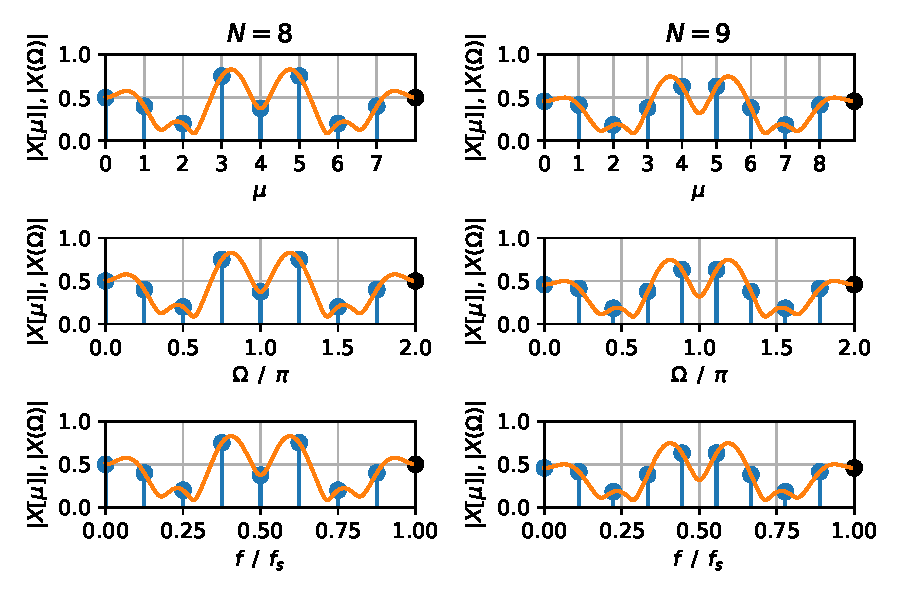
\includegraphics[width=6in, height=4in]{graphics/DTFT_Interpolation.pdf}
		\caption{DFT (stem, blue) and interpolated DTFT (line, red) magnitude
		spectra over $\mu$ (top), $\Omega/\pi$ (middle) and $\frac{f}{f_s}$ (bottom)
		for $N=8$ (left) and $N=9$ (right).}
		\label{DTFT_Interpolation}
\end{figure}
%
As already introduced in eq.~\eqref{eq:OmegaDFT}
%
\begin{equation}
\Omega=\frac{2\pi f}{f_s} \hspace{1cm} \Omega_\text{DFT}=\frac{2\pi f_\text{DFT}}{f_s}
\end{equation}
hold as well.
%
Thus, a DFT and an interpolated DTFT spectrum can be visualised over $\mu$,
$\Omega$ and, for a given sampling frequency $f_s$, over $f$ as depicted in
Fig.~\ref{DTFT_Interpolation}.

% -----------------------------------------------------------------------------
\subsection{Windowing}
Many textbooks treat the derivation of the DFT and windowing separately, which
is sensible if the concept of the DFT is to be introduced solely as a transform.
%
For the spectral analysis of signals, it might be helpful to discuss the DFT
and windowing together as e.g. in \cite{Moeser2011},
\cite[Ch.~7.3,~7.4]{Kammeyer2002}.

Let $x[k]$ for $-\infty\leq k\leq\infty$ be a sequence with the corresponding
continuous and periodic DTFT spectrum $X(\Omega)$.
%
For a computer-assisted spectral analysis, it is necessary to cut out a finite
number of values out of a representative signal section.
%
Mathematically, this is described by multiplication with a weighting or window
sequence $w[k]$, that equals zero outside the desired signal section:
%
\begin{equation}
w[k]=0 \hspace{5mm} \text{for}\,\,k<0\,\,\text{and}\,\,k\geq N, \hspace{5mm} w\in\mathbb{R}.
\end{equation}
%
For example, the definition of a rectangular window is
%
\begin{equation}
w[k]=\left\{\begin{matrix}1 & \text{for} & 0\leq k\leq N-1\\0 & \text{otherwise} &\end{matrix}\right..
\end{equation}
%
Of course the chosen signal section does not have to start at $k=0$,
but it makes calculations easier.
%
The sequence $w[k]$ has a corresponding DTFT spectrum $W(\Omega)$ as well:
%
\begin{align}
W(\Omega)&=\sum_{k=-\infty}^{\infty}w[k]\e^{-\im\Omega k}\nonumber\\
w[k]&=\frac{1}{2\pi}\int\limits_{-\pi}^{\pi}W(\Omega)\e^{\im\Omega k}\text{d}\Omega.
\end{align}
%
Cutting-out the signal section means multiplication of the signal with the
window sequence
%
\begin{equation}
x_\text{N}[k]=x[k]\cdot w[k],
\end{equation}
%
which can be expressed as a cyclic convolution of the corresponding spectra in
the frequency domain:
%
\begin{align}
X_\text{N}(\Omega)&=\frac{1}{2\pi}(X\circledast W)(\Omega)\\
&=\frac{1}{2\pi}\int\limits_{-\pi}^{\pi}X(\Omega-\nu)\cdot W(\nu)\text{d}\nu\\
&= \frac{1}{2\pi}\int\limits_{-\pi}^{\pi}X(\nu)\cdot W(\Omega-\nu)\text{d}\nu.
\end{align}

The DTFT spectrum $X_\text{N}(\Omega)$ contains the "original" DTFT spectrum
$X(\Omega)$ that was to be analysed, but it is smeared due to the convolution
with the window spectrum.
%
The only possibility to obtain $X_\text{N}(\Omega)=X(\Omega)$ is to convolve
with a window that is the neutral element of the convolution
%
\begin{equation}
W_\delta(\Omega)=2\pi\sum_{n=-\infty}^{\infty}\delta(\Omega+2\pi n)
\end{equation}
%
which yields
%
\begin{equation}
X_\text{N}(\Omega)=\int\limits_{-\pi}^{\pi}X(\Omega-\nu)\cdot\delta(\nu)\text{d}\nu
=\int\limits_{-\pi}^{\pi}X(\nu)\cdot\delta(\Omega-\nu)\text{d}\nu=X(\Omega).
\end{equation}
%
However, $W_\delta(\Omega)$ corresponds to \cite[tab.~2.3, p.~90]{Oppenheim2010}
\begin{equation}
W_\delta(\Omega)=2\pi\sum\limits_{n=-\infty}^{\infty}\delta(\Omega+2\pi n) \hspace{5mm}\Laplace\hspace{5mm} w_\delta[k]=1 \hspace{5mm} \text{for}\,\,-\infty\leq k\leq\infty,
\end{equation}
which constitutes an infinitely long window.
%
For the time domain follows
\begin{equation}
x_\text{N}[k]=x[k]\cdot w_\delta[k]=x[k],
\end{equation}
which delivers a consistent theory, but is not helpful for practical computation.

Therefore, $w_\delta[k]$ is not a window that can be employed in practice
(and it is not actually not even a true 'window' as it is constantly 1),
but it should be kept in mind that $W_\delta(\Omega)$ would be the ideal window
spectrum for the analysis of $x[k]$.
%
So we have to accept that instead of being able to analyse $x[k]$ and $X(\Omega)$,
only $x_N[k]$ and $X_\text{N}(\Omega)$ are available.
%
How well $X_\text{N}(\Omega)\approx X(\Omega)$ can be approximated is dependent
on the length $N$ of the cut out section, on the chosen section of $x[k]$ and
on the sequence $w[k]$ and its spectrum $W(\Omega)$, that are itself dependent
on $N$.

To illustrate the importance of the window spectrum, the signal spectrum of a
single harmonic oscillation with the angular frequency $0\leq\Omega_0<\pi$
is considered \cite[tab.~2.3, p.~90]{Oppenheim2010}
%
\begin{equation}
X_\delta(\Omega)=2\pi\sum_{n=-\infty}^{\infty}\delta(\Omega-\Omega_0+2\pi n).
\label{eq:DTFTspec_harmSchwingung}
\end{equation}
%
For $X_\text{N}(\Omega)$ follows from the convolution
$X_{\delta,\text{N}}(\Omega)=\frac{1}{2\pi}(X_\delta\circledast W)(\Omega)$
the spectrum of the window sequence shifted by $\Omega_0$
%
\begin{equation}
X_{\delta,\text{N}}(\Omega)=W(\Omega-\Omega_0).
\end{equation}
%
Therefore, we must be able to interpret the window spectrum to conclude on
$X_\text{N}(\Omega)$ or even $X(\Omega)$.
%
The next section starts discussion on the rectangular window which is the
'natural' window of the DFT definition as it just cuts out a section of the
signal where all values are weighted equally.

%------------------------------------------------------------------------------
\subsubsection{Rectangular Window}
A window $w[k]$ of length $N$ is defined with
%
\begin{equation}
w[k]=0 \hspace{5mm} \text{for}\,\,k<0\,\,\text{and}\,\,k\geq N,\hspace{5mm} w\in\mathbb{R}.
\end{equation}
%
For $0\leq k\leq N-1$, $w[k]$ can consist of arbitrary real numbers.
%
If $w[k]=1$ for this range, a so called rectangular window is obtained.
%
To determine the spectrum of a window, we can calculate the DTFT of the
infinite sequence $w[k]$, where only values of the sequence that are $\neq0$
have to be summed up:
%
\begin{equation}
W(\Omega)=\sum_{k=0}^{N-1}w[k]\cdot\e^{-\im\Omega k}.
\end{equation}
%
For the simple rectangular window this yields
%
\begin{equation}
W_\text{Rect}(\Omega)=\sum_{k=0}^{N-1}1\cdot\e^{-\im\Omega k}.
\label{eq:Ansatz_RectWin}
\end{equation}
%
This is a geometric series for which the closed form solution is known
\cite[(3-39)]{Lyons2011} as
%
\begin{equation}
W_\text{Rect}(\Omega)=\frac{1-\e^{-\im\Omega N}}{1-\e^{-\im\Omega}}.
\end{equation}
%
This expression can be rewritten as
%
\begin{equation}
W_\text{Rect}(\Omega)=\frac{\e^{-\im\frac{\Omega N}{2}}}{\e^{-\im\frac{\Omega}{2}}}\cdot\frac{\e^{\im\frac{\Omega N}{2}}-\e^{-\im\frac{\Omega N}{2}}}{\e^{\im\frac{\Omega}{2}}-\e^{-\im\frac{\Omega}{2}}}
=\e^{-\im\frac{\Omega(N-1)}{2}}\cdot\frac{\e^{\im\frac{\Omega N}{2}}-\e^{-\im\frac{\Omega N}{2}}}{\e^{\im\frac{\Omega}{2}}-\e^{-\im\frac{\Omega}{2}}}
\end{equation}
%
and with the Euler identity $2\im\cdot\sin(x)=\e^{\im x}-\e^{-\im x}$ be
simplified to (cf. \cite[(3-42)]{Lyons2011})
%
\begin{equation}
W_\mathrm{Rect}(\Omega)=\e^{-\im\frac{\Omega(N-1)}{2}}\cdot\frac{\sin\left(N\frac{\Omega}{2}\right)}{\sin\left(\frac{\Omega}{2}\right)}.
\label{eq:DTFT_RectWin}
\end{equation}
%
The spectrum $W_\text{Rect}(\Omega)$ is like all Fourier transformed sequences
$2\pi$-periodic.
%
For the following discussion, only the section of the base band
$-\pi\leq\Omega<\pi$ is considered.

For the magnitude spectrum only the fraction containing the sines has to be
evaluated because $\left|\e^{-\im\frac{\Omega(N-1)}{2}}\right|=1$.
%
With the rule of L'Hospital \cite[(1.4.15	)]{Nist2010} the rectangular
window at $\Omega=0$ is
%
\begin{equation}
W_\text{Rect}(\Omega=0)=N.
\end{equation}
%
This is the amplitude that is weighting the current mid frequency in the
convolution the strongest, the so-called maximum main lobe amplitude.
%
The zeros $W_\text{Rect}(\Omega)=0$ in the base band result with
$m\in\mathbb{Z}$, $m\neq0$ after considering the argument of the sine in the
numerator
%
\begin{equation}
N\frac{\Omega}{2}=m\pi,
\end{equation}
in
\begin{equation}
\Omega=\frac{2\pi}{N}m=\Delta\Omega\cdot m.
\end{equation}
%
The zeros are equidistantly spaced with $\Delta\Omega=\frac{2\pi}{N}$.
%
For odd $N$, $N-1$ zeros result for
\begin{equation}
m=\pm1,\,\pm2,\,\pm3,\,...\,\pm\frac{N-1}{2}.
\end{equation}
%
For even $N$, $N-1$ zeros result for
\begin{equation}
m=\pm1,\,\pm2,\,\pm3,\,...\,\pm\left(\frac{N}{2}-1\right),\,-\frac{N}{2}.
\end{equation}
%
In the last case, the last zero $m=-\frac{N}{2}$ is exactly at $\Omega=-\pi$.
%
As it is a $2\pi$-periodic spectrum this zero could be defined with
$m=\frac{N}{2}$ as $\Omega=\pi$, but this would be the same zero and it is not
counted twice.
%
For $m=0$, no zero can be found, but instead the main lobe, as has been
described above.

Fig.~\ref{RectWindow_DTFT_DFT_lin_asym} and \ref{RectWindow_DTFT_DFT_lin_sym}
illustrate the cases $N=4$ and $N=5$ for the DTFT of the rectangular window.
%
The $N-1$ zeros of the spectrum are clearly visible.
%
Fig.~\ref{RectWindow_DTFT_log_asym} and \ref{RectWindow_DTFT_log_sym} show the
spectra with a logarithmic amplitude.
%
Differing from the depiction here, textbooks mostly use normalised representations
of window spectra of the form $20\cdot\log_{10}W[\Omega=0]=0$~dB, that are
symmetric in $\Omega=0$, i.e. plotted over $-\pi\leq\Omega<\pi$.
%
\begin{figure}
		\centering
		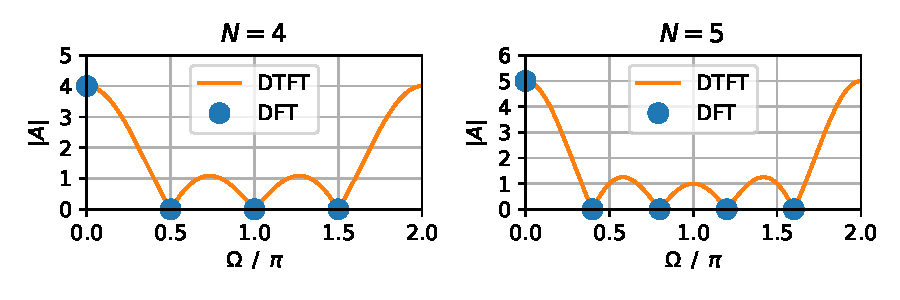
\includegraphics[width=6in, height=2in]{graphics/RectWindow_DTFT_DFT_lin_asym.pdf}
		\caption{Magnitude of DTFT \& DFT spectra for rectangular windows of length
		$N$, $0\leq\Omega<2\pi$.}
		\label{RectWindow_DTFT_DFT_lin_asym}
\end{figure}
\begin{figure}
		\centering
		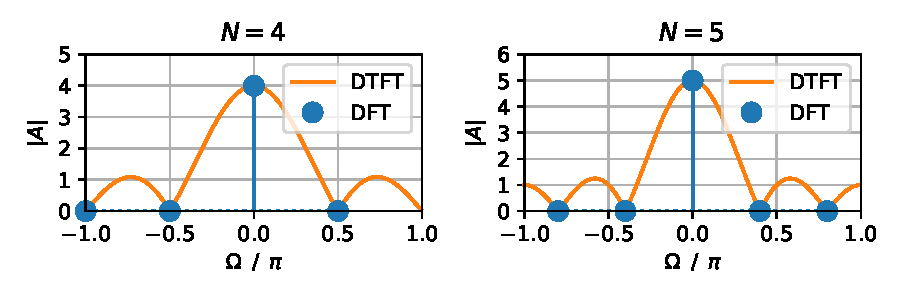
\includegraphics[width=6in, height=2in]{graphics/RectWindow_DTFT_DFT_lin_sym.pdf}
		\caption{Magnitude of DTFT \& DFT spectra for rectangular windows of length
		$N$, $-\pi\leq\Omega<\pi$.}
		\label{RectWindow_DTFT_DFT_lin_sym}
\end{figure}
\begin{figure}
		\centering
		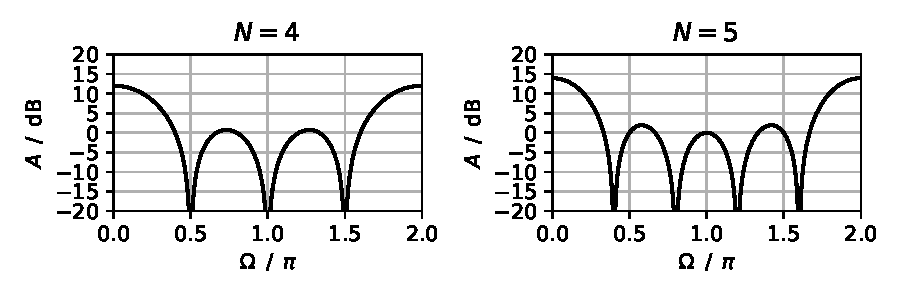
\includegraphics[width=6in, height=2in]{graphics/RectWindow_DTFT_DFT_log_asym.pdf}
		\caption{Level of DTFT spectra for rectangular windows of length $N$,
		$0\leq\Omega<2\pi$.}
		\label{RectWindow_DTFT_log_asym}
\end{figure}
\begin{figure}
		\centering
		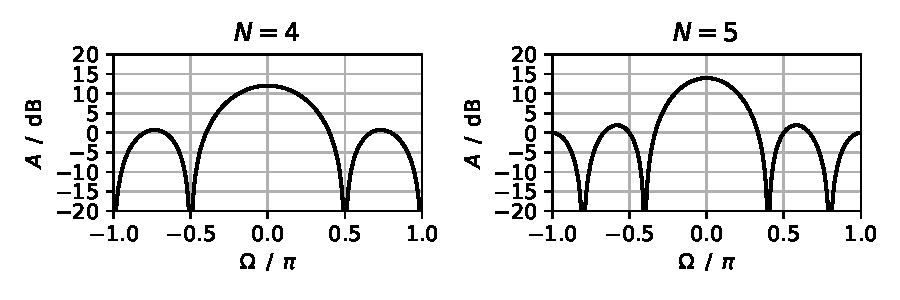
\includegraphics[width=6in, height=2in]{graphics/RectWindow_DTFT_DFT_log_sym.pdf}
		\caption{Level of DTFT spectra for rectangular windows of length $N$,
		$-\pi\leq\Omega<\pi$.}
		\label{RectWindow_DTFT_log_sym}
\end{figure}

%------------------------------------------------------------------------------
\subsubsection{Discrete Spectrum of the Rectangular Window}
As has been explained before, the spectrum from eq.~\eqref{eq:DTFTspec_harmSchwingung}
%
\begin{equation}
X_\delta(\Omega)=2\pi\sum\limits_{n=-\infty}^\infty\delta(\Omega-\Omega_0+2\pi n)
\end{equation}
%
evolves with windowing, i.e. the convolution
$X_{\delta,\text{N}}(\Omega)=\frac{1}{2\pi}\,(X_\delta\circledast W)(\Omega)$,
into
%
\begin{equation}
X_{\delta,\text{N}}(\Omega)=W(\Omega-\Omega_0).
\end{equation}
%
Now, the spectrum of a finite signal is considered, i.e. a transition from the
DTFT to the DFT is performed.
%
For the discrete DFT frequencies that contain the complete spectral information,
$X_\delta[\mu]$ can be written as
%
\begin{equation}
X_\delta[\mu]=W\left[\frac{2\pi}{N}\mu-\Omega_0\right].
\end{equation}
%
With eq.~\eqref{eq:DTFT_RectWin} follows
%
\begin{align}
X_\delta[\mu]=W_\text{Rect}\left[\frac{2\pi}{N}\mu-\Omega_0\right]&=\e^{-\im\frac{\left(\frac{2\pi}{N}\mu-\Omega_0\right)(N-1)}{2}}\cdot\frac{\sin\left(N\frac{\frac{2\pi}{N}\mu-\Omega_0}{2}\right)}{\sin\left(\frac{\frac{2\pi}{N}\mu-\Omega_0}{2}\right)}\\
&=\e^{-\im\left(\frac{N-1}{2}\left(\frac{2\pi}{N}\mu-\Omega_0\right)\right)}\cdot\frac{\sin\left(\frac{N}{2}\left(\frac{2\pi}{N}\mu-\Omega_0\right)\right)}{\sin\left(\frac{1}{2}\left(\frac{2\pi}{N}\mu-\Omega_0\right)\right)}.
\label{eq:DFTspec_RectWin}
\end{align}
%
As can be seen, the DFT coefficients $X_\delta[\mu]$ strongly depend on
the choice of $\Omega_0$, which will be illustrated in the following.
%
The definition
%
\begin{equation}
\Omega_0=\frac{2\pi}{N}(\mu_0+\alpha)
\hspace{5mm} \text{with} \hspace{5mm}
\pm\alpha\leq\frac{1}{2}
\end{equation}
%
is inserted into eq.~\eqref{eq:DFTspec_RectWin} to yield
%
\begin{align}
X_\delta[\mu]&=\e^{-\im\left(\frac{N-1}{2}\left(\frac{2\pi}{N}\mu-\frac{2\pi}{N}(\mu_0+\alpha)\right)\right)}\cdot\frac{\sin\left(\frac{N}{2}\left(\frac{2\pi}{N}\mu-\frac{2\pi}{N}(\mu_0+\alpha)\right)\right)}{\sin\left(\frac{1}{2}\left(\frac{2\pi}{N}\mu-\frac{2\pi}{N}(\mu_0+\alpha)\right)\right)}\\
&=\e^{-\im\left(\frac{N-1}{2}\left(\frac{2\pi}{N}(\mu-\mu_0)-\frac{2\pi}{N}\alpha\right)\right)}\cdot\frac{\sin\left(\pi((\mu-\mu_0)-\alpha)\right)}{\sin\left(\frac{\pi}{N}((\mu-\mu_0)-\alpha)\right)}.
\label{eq:DFTspec_mitalpha}
\end{align}
%
For the case $\alpha=0$, we have $\Omega_0=\frac{2\pi}{N}\mu_0$ and the fraction
containing the sines evaluates to $N$ (cf. periodic sinc in
eq.~\eqref{eq:periodic_sinc}), so the DFT spectrum becomes
%
\begin{equation}
X_\delta[\mu]=\left\{\begin{matrix}0 & \text{for} & \mu\neq\mu_0\\N & \text{for} & \mu=\mu_0\end{matrix}\right..
\end{equation}
%
Therefore, if the chosen frequency from eq.~\eqref{eq:DTFTspec_harmSchwingung}
happens to be a DFT bin, the frequency spectrum contains the exact amplitude of
this frequency (after normalising with $\frac{1}{N}$).
%
The other values of the spectrum coincide with the zeros of the window spectrum.
%
This is the best case because the amplitude of the frequency $\Omega_0$ can be
analysed exactly, cf. Fig.~\ref{DFTbestworstcase_RectWin} left.
%
The worst case occurs when $\alpha=\pm\frac{1}{2}$.
%
For the rectangular window, two bins share the main energy and the other bins
differ from zero as well, cf. Fig.~\ref{DFTbestworstcase_RectWin} right.
%
It is not as easy anymore how to interpret the DFT spectrum.
%
From the example it is known that the signal consists of only one spectral
component, but in the spectrum this is not so obvious.
%
So what is to do when the frequencies and corresponding amplitudes of the signal
are not known (as is of course usually the case in real applications)?
%
\begin{figure}
		\centering
		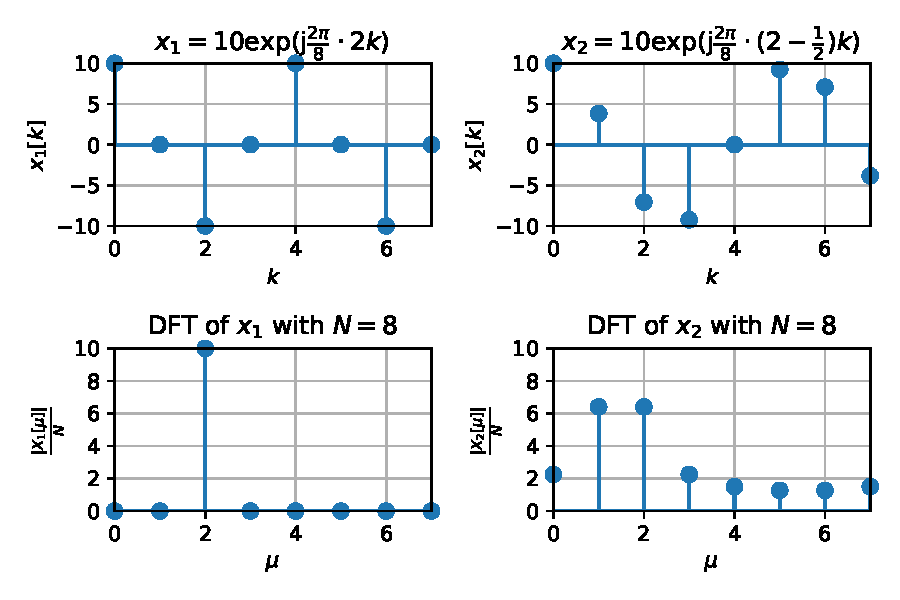
\includegraphics[width=6in, height=4in]{graphics/DFTbestworstcase_RectWin.pdf}
		\caption{Rectangular windowing for $N=8$,
		best case ($\mu=2$), worst case ($\mu=2-\frac{1}{2}$).}
		\label{DFTbestworstcase_RectWin}
\end{figure}

For the interpretation of such spectra, knowledge about windowing and different
window types as well as experience in analysing spectra is necessary.
%
In a first step we can determine for each window which amplitude error arises
between best and worst case.
%
This gives an indication for the "true" spectrum.
%
For the rectangular window, this calculation is quite easy and is shown here:
%
With eq.~\eqref{eq:DFTspec_mitalpha}, the amplitude for a certain $\mu_0$ is
generally
%
\begin{equation}
|X_\delta[\mu_0]|=\left|\frac{\sin(-\pi\alpha)}{\sin\left(-\frac{\pi}{N}\alpha\right)}\right|
=\left|\frac{\sin(\pi\alpha)}{\sin\left(\frac{\pi}{N}\alpha\right)}\right|
\end{equation}
%
and for the worst case $\alpha=\pm\frac{1}{2}$
%
\begin{equation}
|X_\delta[\mu_0]|=\left|\frac{\sin\left(\pm\frac{\pi}{2}\right)}{\sin\left(\pm\frac{\pi}{2N}\right)}\right|
=\left|\frac{\pm1}{\pm\sin\left(\frac{\pi}{2N}\right)}\right|
=\left|\frac{1}{\sin\left(\frac{\pi}{2N}\right)}\right|.
\end{equation}
%
For very large $N$, this yields due to $\sin(x)\approx x$ for small $x$ the
amplitude
%
\begin{equation}
|X_\delta[\mu_0]|=\frac{2N}{\pi}.
\end{equation}
%
The amplitude error between the best case for $\alpha=0$ and the worst case for
$\alpha=\pm\frac{1}{2}$ is then for large $N$
%
\begin{equation}
\frac{\left|X_\delta[\mu_0]_{\alpha=\pm\frac{1}{2}}\right|}{\left|X_\delta[\mu_0]_{\alpha=0}\right|}\approx\frac{\frac{2N}{\pi}}{N}\approx\frac{2}{\pi}\approx0.6366\,\hat{=}\,-3.9224\,\text{dB}.
\end{equation}
%
The amplitude loss from the value 10 to approx. 6.3 can be found in
Fig.~\ref{DFTbestworstcase_RectWin}.
%
It is still not known, though, which frequencies the signal consists of
($\mu=1$ or $\mu=2$ or both?).
%
This could be accomplished by an increase of $N$.
%
Additionally, the quite high amplitudes in the other bins are confusing.
%
This point can be counteracted with a window with a higher side lobe
attenuation that is presented in the next subsection discussing the Hann
window.

%------------------------------------------------------------------------------
\subsubsection{Hann Window}
\begin{figure}
		\centering
		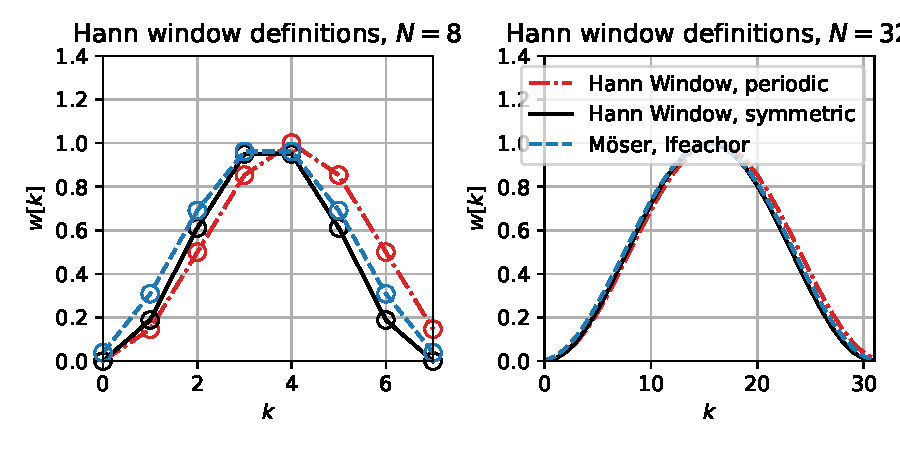
\includegraphics[width=6in, height=3in]{graphics/HannDefinitionen.pdf}
		\caption{Different definitions of the Hann window.}
		\label{HannDefinitionen}
\end{figure}

For the Hann window (and for other windows as well), different definitions
exist in the literature.
%
Fig.~\ref{HannDefinitionen} shows differently defined Hann windows for two
lengths $N$.
%
The red line starts at $w[k=0]=0$, but ends with $w[k=N-1]\neq0$.
%
This is based upon the reason that (at least for spectral analysis) a symmetric
window is not necessary \cite[p.~52]{Harris1978}.
%
Instead, the window is constructed in a such a way that for periodic extension
$w[N]=w[0]$.
%
The black line defines a window that is symmetric around $\frac{N-1}{2}$ and at
both terminal points $w[k=0]=0$ and $w[k=N-1]=0$ holds, because of the common
reasoning that the windowed signal must be zero at the terminal points to
ensure continuous transitions for periodic repetitions
\cite{Oppenheim2010, Lyons2011}.
%
The blue curve defines a window that is symmetric around $\frac{N-1}{2}$ as well,
but both terminal points $w[k=0]\neq0$ and $w[k=N-1]\neq0$.
%
The reason for this is that $N$ `real' DFT bins should be retrieved
\cite{Moeser2011, Ifeachor2002}.
%
This is why the sequence $w[k]$ for the blue line consists of $N$ coefficients
that differ from 0 while it is only $N-2$ for the black line.
%
A DFT of length $N$ for a sequence with only $N-2$ coefficients differing from
0 yields only $N-2$ `real' bins (compare to zero-padding).
%
For scientific purposes, it should be stated which definition of a standard
window has been used.

The application can determine which definition of a window is appropriate.
%
For spectral analysis a window should be used that can be extended periodically
without losing information in bins.
%
Those windows do not have to be symmetric around the middle of the window.
%
In FIR filter design we aim at reducing an infinite impulse response to a
finite length.
%
This is mostly done by symmetric windows to window symmetrically around the main
peak of the impulse response.
%
Therefore, Matlab and Python discriminate between the variants \texttt{periodic} and
\texttt{symmetric},  \texttt{symmetric=True/False} respectively in window design.

Although the Matlab window as \texttt{periodic} version would be better suited
for storytelling, for the following, the window definition of \cite{Moeser2011}
is used, since the manual calculation is more convenient.
%
For the window $w[k]$ of length $N$,
%
\begin{equation}
w[k]=0 \hspace{5mm} \text{for}\,\,k<0\,\,\text{and}\,\,k\geq N,
\hspace{5mm} w\in\mathbb{R}
\end{equation}
%
is still valid.
%
For $0\leq k\leq N-1$, $w[k]$ shall consist of arbitrary real numbers.
%
In this case here, those numbers are the ones of a Hann window.
%
Additionally, the window should be symmetric
%
\begin{equation}
w[N-1-k]=w[k]
\end{equation}
%
and without zeros in the definition range.
%
The Hann window version that fulfills this requirement reads
%
\begin{align}
w[k]=\left\{\begin{matrix}1-\cos\left(\frac{2\pi}{N}\left(k+\frac{1}{2}\right)\right) & \text{for} & 0\leq k\leq N-1\\0 & \text{else} & \end{matrix}\right..
\label{eq:hanning}
\end{align}
%
The spectrum can be calculated with the help of
\begin{equation}
\cos\left(\frac{2\pi}{N}\left(k+\frac{1}{2}\right)\right)=\frac{1}{2}\left(\e^{\im\frac{\pi}{N}}\e^{\im\frac{2\pi}{N}k}+\e^{-\im\frac{\pi}{N}}\e^{-\im\frac{2\pi}{N}k}\right)
\end{equation}
%
and
%
\begin{equation}
W(\Omega)=\sum\limits_{k=0}^{N-1}w[k]\e^{-\im\Omega k}.
\end{equation}
%
Therefore, the spectrum of the window is
%
\begin{align}
W_{\text{Hann}}(\Omega)&=\sum\limits_{k=0}^{N-1}\left(1-\cos\left(\frac{2\pi}{N}\left(k+\frac{1}{2}\right)\right)\right)\e^{-\im\Omega k}\\
&=\sum\limits_{k=0}^{N-1}\left(1-\frac{1}{2}\left(\e^{\im\frac{\pi}{N}}\e^{\im\frac{2\pi}{N}k}+\e^{-\im\frac{\pi}{N}}\e^{-\im\frac{2\pi}{N}k}\right)\right)\e^{-\im\Omega k}\\
&=\sum\limits_{k=0}^{N-1}\e^{-\im\Omega k}-\frac{1}{2}\e^{\im\frac{\pi}{N}}\sum\limits_{k=0}^{N-1}\e^{-\im\left(\Omega-\frac{2\pi}{N}\right)k}-\frac{1}{2}\e^{-\im\frac{\pi}{N}}\sum\limits_{k=0}^{N-1}\e^{-\im\left(\Omega+\frac{2\pi}{N}\right)k}.
\end{align}
%
Using the results for the rectangular windows
(cf. eq.~\eqref{eq:Ansatz_RectWin}), this can be abbreviated to
%
\begin{equation}
W_{\text{Hann}}(\Omega)=W_{\text{Rect}}(\Omega)-\frac{1}{2}\e^{\im\frac{\pi}{N}}W_{\text{Rect}}(\Omega-\frac{2\pi}{N})-\frac{1}{2}\e^{-\im\frac{\pi}{N}}W_{\text{Rect}}(\Omega+\frac{2\pi}{N}).
\end{equation}
%
As can be seen, the spectrum of the Hann window is composed of the spectrum
of a rectangular window and two weighted spectra of rectangular windows
that are shifted by one bin.
%
With eq.~\eqref{eq:DTFT_RectWin}, this can be rewritten as
%
\begin{align}
W_{\text{Hann}}(\Omega)=&\e^{-\im\frac{\Omega(N-1)}{2}}\cdot\frac{\sin\left(N\frac{\Omega}{2}\right)}{\sin\left(\frac{\Omega}{2}\right)}\nonumber\\
&-\frac{1}{2}\e^{\im\frac{\pi}{N}}\e^{-\im\frac{(\Omega-\frac{2\pi}{N})(N-1)}{2}}\cdot\frac{\sin\left(N\frac{\Omega-\frac{2\pi}{N}}{2}\right)}{\sin\left(\frac{\Omega-\frac{2\pi}{N}}{2}\right)}\nonumber\\
&-\frac{1}{2}\e^{-\im\frac{\pi}{N}}\e^{-\im\frac{(\Omega+\frac{2\pi}{N})(N-1)}{2}}\cdot\frac{\sin\left(N\frac{\Omega+\frac{2\pi}{N}}{2}\right)}{\sin\left(\frac{\Omega+\frac{2\pi}{N}}{2}\right)}\\
=&\e^{-\im\frac{\Omega(N-1)}{2}}\cdot\frac{\sin\left(\frac{N}{2}\Omega\right)}{\sin\left(\frac{1}{2}\Omega\right)}\nonumber\\
&-\frac{1}{2}\e^{\im\frac{\pi}{N}}\e^{-\im\frac{(\Omega-\frac{2\pi}{N})(N-1)}{2}}\cdot\frac{\sin\left(\frac{N}{2}\left(\Omega-\frac{2\pi}{N}\right)\right)}{\sin\left(\frac{1}{2}\left(\Omega-\frac{2\pi}{N}\right)\right)}\nonumber\\
&-\frac{1}{2}\e^{-\im\frac{\pi}{N}}\e^{-\im\frac{(\Omega+\frac{2\pi}{N})(N-1)}{2}}\cdot\frac{\sin\left(\frac{N}{2}\left(\Omega+\frac{2\pi}{N}\right)\right)}{\sin\left(\frac{1}{2}\left(\Omega+\frac{2\pi}{N}\right)\right)}.
\end{align}
%
Because
%
\begin{equation}
\e^{\im\frac{\pi}{N}}\e^{-\im\frac{(\Omega-\frac{2\pi}{N})(N-1)}{2}}=\e^{-\im\frac{\Omega(N-1)}{2}}\e^{\im\frac{\pi}{N}}\e^{\im\frac{(N-1)}{2}\frac{2\pi}{N}}
=\e^{-\im\frac{\Omega(N-1)}{2}}\underbrace{\e^{\im\pi\left(\frac{1}{N}+\frac{N-1}{N}\right)}}_{=-1}
\end{equation}
%
and
%
\begin{equation}
\e^{-\im\frac{\pi}{N}}\e^{-\im\frac{(\Omega+\frac{2\pi}{N})(N-1)}{2}}=\e^{-\im\frac{\Omega(N-1)}{2}}\e^{-\im\frac{\pi}{N}}\e^{-\im\frac{(N-1)}{2}\frac{2\pi}{N}}
=\e^{-\im\frac{\Omega(N-1)}{2}}\underbrace{\e^{-\im\pi\left(\frac{1}{N}+\frac{N-1}{N}\right)}}_{=-1},
\end{equation}
%
the spectrum can be simplified to
%
\begin{align}
W_{\text{Hann}}(\Omega)&=\e^{-\im\frac{\Omega(N-1)}{2}}\cdot\frac{\sin\left(\frac{N}{2}\Omega\right)}{\sin\left(\frac{1}{2}\Omega\right)}+\frac{1}{2}\e^{-\im\frac{\Omega(N-1)}{2}}\cdot\frac{\sin\left(\frac{N}{2}\left(\Omega-\frac{2\pi}{N}\right)\right)}{\sin\left(\frac{1}{2}\left(\Omega-\frac{2\pi}{N}\right)\right)}+\frac{1}{2}\e^{-\im\frac{\Omega(N-1)}{2}}\cdot\frac{\sin\left(\frac{N}{2}\left(\Omega+\frac{2\pi}{N}\right)\right)}{\sin\left(\frac{1}{2}\left(\Omega+\frac{2\pi}{N}\right)\right)}\\
&=\e^{-\im\frac{\Omega(N-1)}{2}}\cdot\left(\frac{\sin\left(\frac{N}{2}\Omega\right)}{\sin\left(\frac{1}{2}\Omega\right)}+\frac{1}{2}\cdot\frac{\sin\left(\frac{N}{2}\left(\Omega-\frac{2\pi}{N}\right)\right)}{\sin\left(\frac{1}{2}\left(\Omega-\frac{2\pi}{N}\right)\right)}+\frac{1}{2}\cdot\frac{\sin\left(\frac{N}{2}\left(\Omega+\frac{2\pi}{N}\right)\right)}{\sin\left(\frac{1}{2}\left(\Omega+\frac{2\pi}{N}\right)\right)}\right).
\end{align}

The Hann window exhibits only $N-3$ zeros compared to the rectangular window
with $N-1$ zeros, so two zeros are lost for usage in spectral shaping,
cf. fig~\ref{HanningausRectWindow} and \ref{DTFTHanningWin_lin}.
%
In the region close to $\Omega=\pm\pi$, the weighted and shifted spectra of
the rectangular windows (red and dark blue line) cancel out, which can be
observed in the logarithmic depiction in Fig.~\ref{DTFTHanningWin_log} as well,
i.e. the Hann window achieves a better side lobe attenuation than the
rectangular window.
%
Around $\Omega\approx 0$, all three spectral components add up in a constructive
way, which leads to a broader main lobe compared to the rectangular window.
%It is worth to realize that no window can have a narrower main lobe than the rect
%window.

\begin{figure}
		\centering
		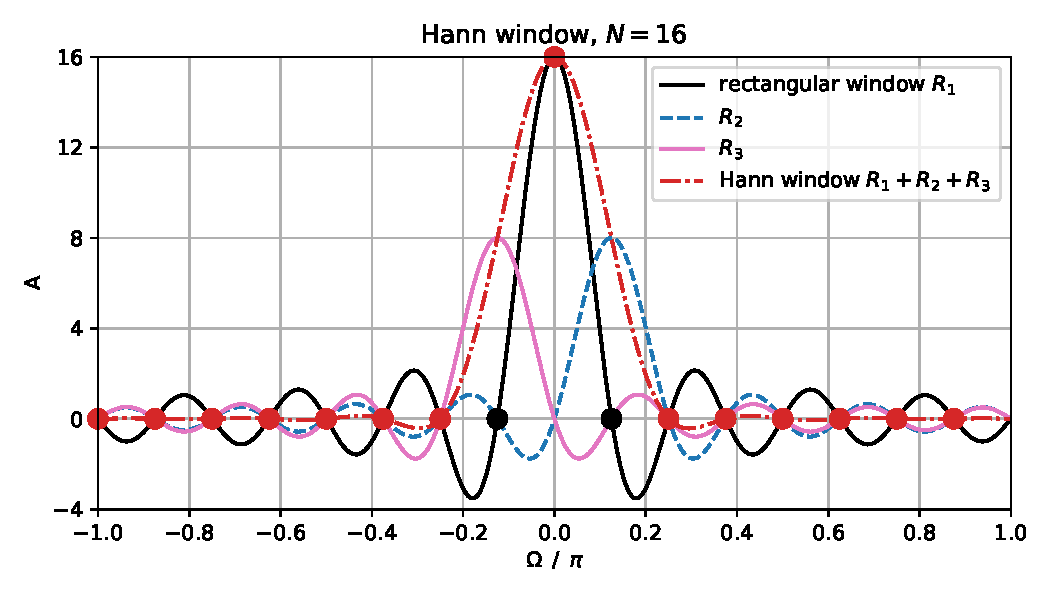
\includegraphics[width=6in, height=3.5in]{graphics/Hann_from_RectWindow.pdf}
		\caption{Spectrum of Hann window from superposition of weighted rectangular windows.}
		\label{HanningausRectWindow}
\end{figure}
\begin{figure}
		\centering
		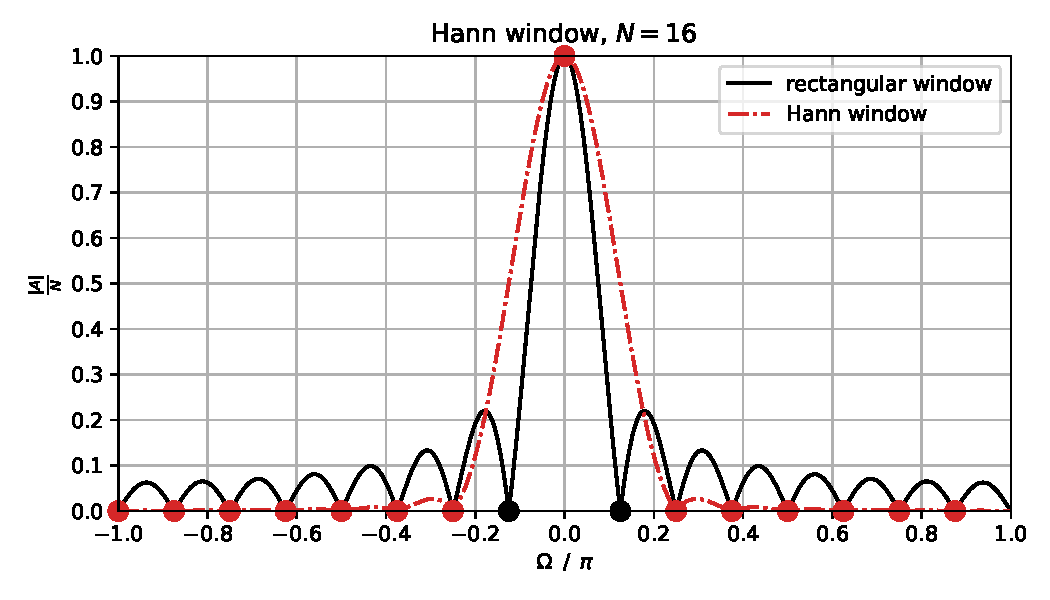
\includegraphics[width=6in, height=3.5in]{graphics/DTFTHannWin_lin.pdf}
		\caption{Magnitude of DTFT spectra for rectangular and Hann window, $-\pi\leq\Omega<\pi$.}
		\label{DTFTHanningWin_lin}
\end{figure}
\begin{figure}
		\centering
		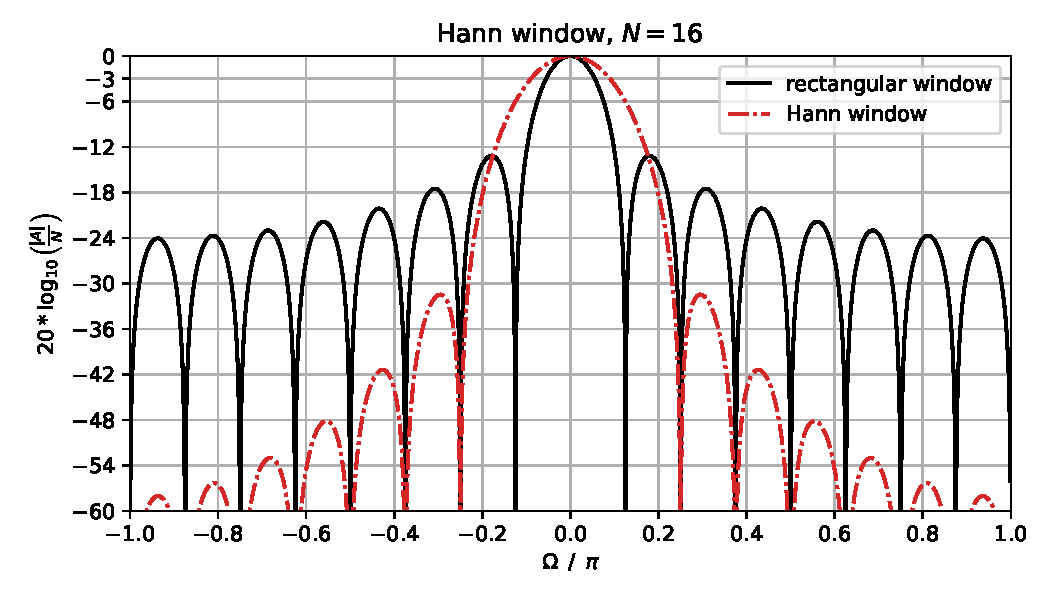
\includegraphics[width=6in, height=3.5in]{graphics/DTFTHannWin_log.pdf}
		\caption{Level of DTFT spectra for rectangular and Hann window, $-\pi\leq\Omega<\pi$.}
		\label{DTFTHanningWin_log}
\end{figure}
\begin{figure}
		\centering
		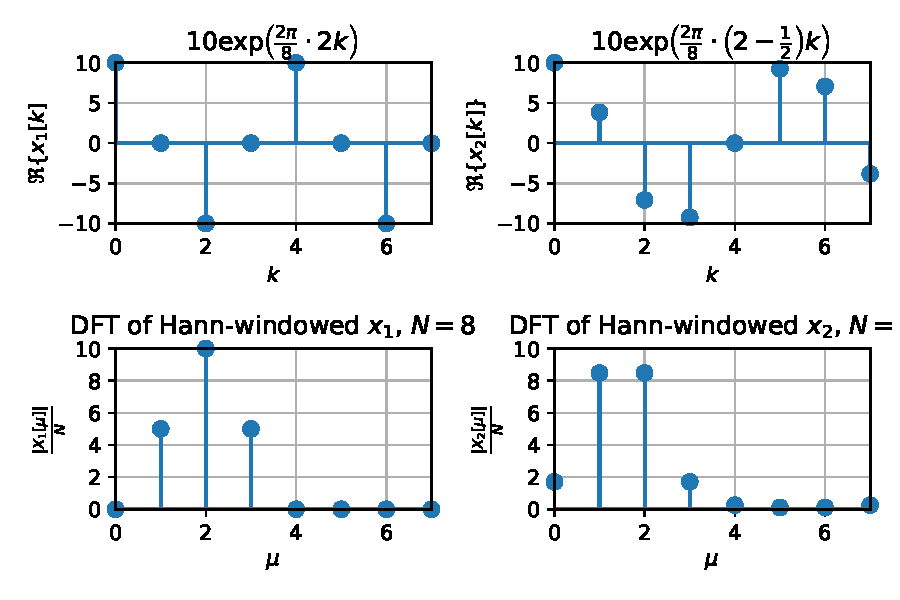
\includegraphics[width=6in, height=4in]{graphics/DFTbestworstcase_HannWin.pdf}
		\caption{Hann windowing for $N=8$, best case ($\mu=2$), worst case ($\mu=2-\frac{1}{2}$).}
		\label{DFTbestworstcase_HannWin}
\end{figure}

Fig.~\ref{DFTbestworstcase_HannWin} illustrates the best and worst case
scenarios for the Hann window when a discrete frequency exactly coincides
with a DFT bin (left, best) or lies in the middle between two bins (right, worst).
%
In contrast to the rectangular window, the exact case ($\mu=2$, left) leads to
three bins that are differing from zero with the middle bin representing the
exact amplitude of the discrete frequency.
%
The worst case ($\mu=2-\frac{1}{2}$, right) leads to two main bins and further
bins differing from zero.
%
The amplitude error between best and worst case for large $N$ is
%
\begin{equation}
\frac{\left|X[\mu_0]_{\alpha=\pm\frac{1}{2}}\right|}{\left|X[\mu_0]_{\alpha=0}\right|}=\frac{3\pi}{8}\approx1.1781\,\hat{=}\,-1.4236\,\text{dB},
\end{equation}
%
which is smaller than the error for the rectangular window.
%
This discloses the following general rule: The broader the main lobe of a window,
the smaller the amplitude error in spectral analysis for a harmonic signal with
the frequency
%
\begin{equation}
\Omega_0=\frac{2\pi}{N}(\mu_0+\alpha) \hspace{5mm} \text{with} \hspace{5mm} \pm\alpha\leq\frac{1}{2}.
\end{equation}
%
However, a broad main lobe leads to a poor frequency resolution, i.e.
frequencies that are close together get smeared in the convolution process
$X_N(\Omega)=\frac{1}{2\pi}(X_N\circledast W)(\Omega)$ and cannot be separated
clearly anymore. So, there is always a compromise involved in frequency
resolution and amplitude accuracy.

One last remark on the amplitudes of the windows: In the literature, windows
are often normalised to a maximum value $=1$, which reads for
the Hann window according to \cite{Moeser2011}
%
\begin{align}
w[k]=\left\{\begin{matrix}0.5-0.5\cos\left(\frac{2\pi}{N}\left(k+\frac{1}{2}\right)\right) & \text{for} & 0\leq k\leq N-1\\0 & \text{else} &\end{matrix}\right..
\end{align}
%
The definition that has been used above (cf. eq.~\eqref{eq:hanning}),
\begin{align}
w[k]=\left\{\begin{matrix}1-\cos\left(\frac{2\pi}{N}\left(k+\frac{1}{2}\right)\right) & \text{for} & 0\leq k\leq N-1\\0 & \text{else} &\end{matrix}\right..
\end{align}
was chosen to result in equal amplitudes $N$ for the rectangular and the Hann
window.
%
In the classic paper \cite[tab.~1]{Harris1978} this normalisation
factor is treated as the so-called `coherent gain'.

%------------------------------------------------------------------------------
\subsubsection{Hamming Window}
The Hann window with only $N-3$ zeros in its spectrum lets two potential
zeros unused.
%
Note that using all possible $N$ zeros would not allow to create a distinct main
lobe at $\Omega=0$, therefore only $N-1$ zeros are used for optimal window
design.
%
The Hamming window adds these zeros again to the Hann window spectrum in
order to improve the attenuation of the first side lobes (left and right of
the main lobe).
%
To that end, the Hann window spectrum is modified with a factor $\beta$ (cf.
\cite[Ch. 3.10]{Rabiner1975}):
%
\begin{equation}
W_{\text{Hamm}}(\Omega)=\e^{-\im\frac{\Omega(N-1)}{2}}\cdot\left(\frac{\sin\left(\frac{N}{2}\Omega\right)}{\sin\left(\frac{1}{2}\Omega\right)}+\frac{\beta}{2}\cdot\frac{\sin\left(\frac{N}{2}\left(\Omega-\frac{2\pi}{N}\right)\right)}{\sin\left(\frac{1}{2}\left(\Omega-\frac{2\pi}{N}\right)\right)}+\frac{\beta}{2}\cdot\frac{\sin\left(\frac{N}{2}\left(\Omega+\frac{2\pi}{N}\right)\right)}{\sin\left(\frac{1}{2}\left(\Omega+\frac{2\pi}{N}\right)\right)}\right).
\end{equation}
%
At $\Omega=\frac{2\pi}{N}\cdot2.5$, i.e. at $\mu=2.5$ in the DFT spectrum, an
additional zero shall be inserted at the maximum of the first side lobe.
%
As $w[k]$ shall be real, this zero must have a symmetric counterpart (so this
yields the desired two additional zeros), but only one has to be specified.
%
For small arguments, the approximation $\sin(x)\approx x$ holds, which is
fulfilled in the denominators for large $N$ when $\Omega=\frac{2\pi}{N}\cdot2.5$,
and for $\Omega=5\pi/N$ the result is:
%
\begin{equation}
\left|W_{\text{Hamm}}(\Omega=\frac{5\pi}{N})\right|\approx\left|\frac{\sin\left(\frac{N}{2}\frac{5\pi}{N}\right)}{\frac{1}{2}\frac{5\pi}{N}}+\frac{\beta}{2}\cdot\frac{\sin\left(\frac{N}{2}\left(\frac{5\pi}{N}-\frac{2\pi}{N}\right)\right)}{\frac{1}{2}\left(\frac{5\pi}{N}-\frac{2\pi}{N}\right)}+\frac{\beta}{2}\cdot\frac{\sin\left(\frac{N}{2}\left(\frac{5\pi}{N}+\frac{2\pi}{N}\right)\right)}{\frac{1}{2}\left(\frac{5\pi}{N}+\frac{2\pi}{N}\right)}\right|.
\end{equation}
%
Searching for the zero
%
\begin{equation}
\left|W_{\text{Hamm}}(\Omega=\frac{5\pi}{N})\right|=\left|\frac{1}{\frac{5\pi}{2N}}+\frac{\beta}{2}\cdot\frac{-1}{\frac{3\pi}{2N}}+\frac{\beta}{2}\cdot\frac{-1}{{\frac{7\pi}{2N}}}\right|\stackrel{!}{=}0
\end{equation}
%
and solving for the corresponding $\beta$ yields
%
\begin{align}
\frac{\beta}{2}\cdot\left(\frac{2N}{3\pi}+\frac{2N}{7\pi}\right)&=\frac{2N}{5\pi}\\
\Leftrightarrow \hspace{5mm} \beta&=\frac{21}{25}=0.84.
\end{align}
%
The Hamming window can be rearranged to
%
\begin{equation}
W_{\text{Hamm}}(\Omega) = (1-\beta)\,W_{\text{Rect}}(\Omega) + \beta\,W_{\text{Hann}}(\Omega),
\end{equation}
%
which means for the sequence
%
\begin{equation}
w_{\text{Hamm}}[k]=\left\{\begin{matrix}(1-\beta)w_{\text{Rect}}[k]+\beta\,w_{\text{Hann}}[k] & \text{for} & 0\leq k\leq N-1\\0 & \text{else} &\end{matrix}\right.
\end{equation}
%
with
%
\begin{equation}
w_{\text{Rect}}[k]=\left\{\begin{matrix}1 & \text{for} & 0\leq k\leq N-1\\0 & \text{else} &\end{matrix}\right.
\end{equation}
%
and
%
\begin{equation}
w_{\text{Hann}}[k]=\left\{\begin{matrix}1-\cos\left(\frac{2\pi}{N}\left(k+\frac{1}{2}\right)\right) & \text{for} & 0\leq k\leq N-1\\0 & \text{else} &\end{matrix}\right..
\end{equation}
%
Finally, the sequence of the Hamming window can be rewritten to
%
\begin{equation}
w_{\text{Hamm}}[k]=\left\{\begin{matrix}1-0.84\cos\left(\frac{2\pi}{N}\left(k+\frac{1}{2}\right)\right) & \text{for} & 0\leq k\leq N-1\\0 & \text{else} &\end{matrix}\right..
\end{equation}
%
The derivation from \cite[p.~62]{Harris1978} concludes that the Hamming window
as it is defined in the standard literature must have been developed by
rounding, which means that the zero is at $\Omega\approx\frac{2\pi}{N}\cdot2.6$.
%
If this zero is used in the calculation here according to \cite{Moeser2011},
$\beta\approx0.852$ results.
%
If now the windows are scaled to have a maximum of 1 for odd $N$, the common
representation of the Hamming window in the literature results
(here written in the form of \cite{Moeser2011}):
%
\begin{align}
w_{\text{Hamm}}[k]&\approx0.54-0.54\,\beta\cdot\cos\left(\frac{2\pi}{N}\left(k+\frac{1}{2}\right)\right)\\
&=0.54-0.46\cdot\cos\left(\frac{2\pi}{N}\left(k+\frac{1}{2}\right)\right).
\end{align}

Fig.~\ref{HammingausRectWindow} shows the additionally added zeros which leads
to strongly attenuated first side lobes visible in the logarithmic spectrum in
Fig.~\ref{DTFTHammingWin_log}.
%
Fig.~\ref{DTFTRectHanningHammingWin_log} displays a comparison of the
rectangular, Hann and Hamming window.
%
It shows that the strongly attenuated first side lobes of the Hamming window
are traded for a slower decrease of the side lobes, but the main lobe is
slightly narrower than for the Hann window.
%
Fig.~\ref{DFTbestworstcase_HammWin} shows the best and worst case scenario for
a Hamming window with $\beta=0.84$.
%
Compared to the Hann window the secondary maxima are lower, but the
amplitude error in the worst case is larger.
%
It is approx.~$-1.78$~dB and is termed "scalloping loss" in \cite{Harris1978}.
\begin{figure}
		\centering
		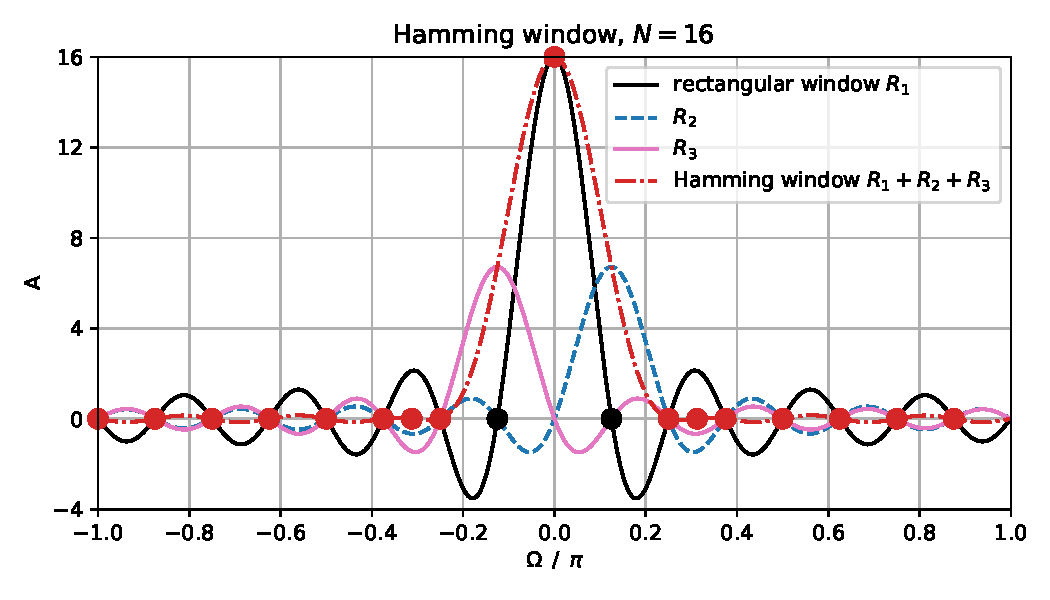
\includegraphics[width=6in, height=3.5in]{graphics/Hamming_from_RectWindow.pdf}
		\caption{Spectrum of Hamming window from superposition of weighted
		rectangular windows.}
		\label{HammingausRectWindow}
\end{figure}
\begin{figure}
		\centering
		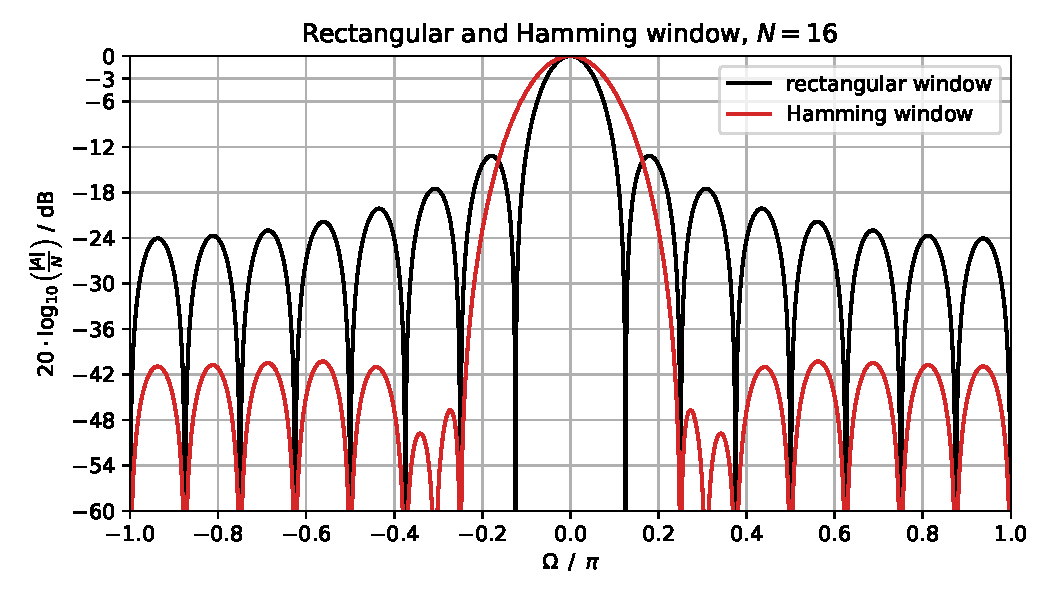
\includegraphics[width=6in, height=3.5in]{graphics/DTFTHammingWin_log.pdf}
		\caption{Level of DTFT spectra for rectangular and Hamming window.}
		\label{DTFTHammingWin_log}
\end{figure}
\begin{figure}
		\centering
		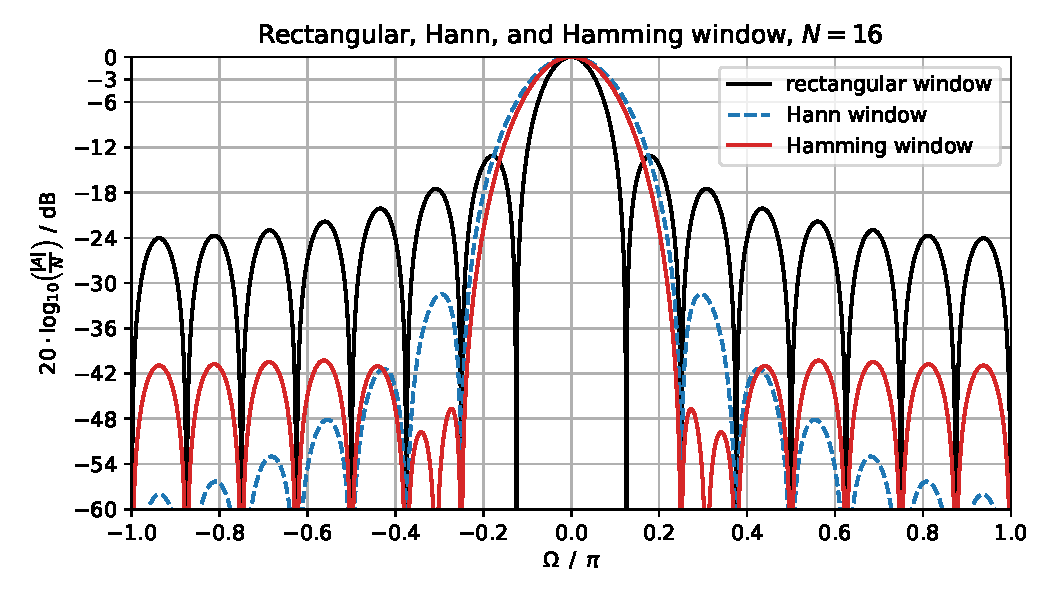
\includegraphics[width=6in, height=3.5in]{graphics/DTFTRectHanningHammingWin_log.pdf}
		\caption{Level of DTFT spectra for rectangular, Hann and Hamming
		window.}
		\label{DTFTRectHanningHammingWin_log}
\end{figure}
\begin{figure}
		\centering
		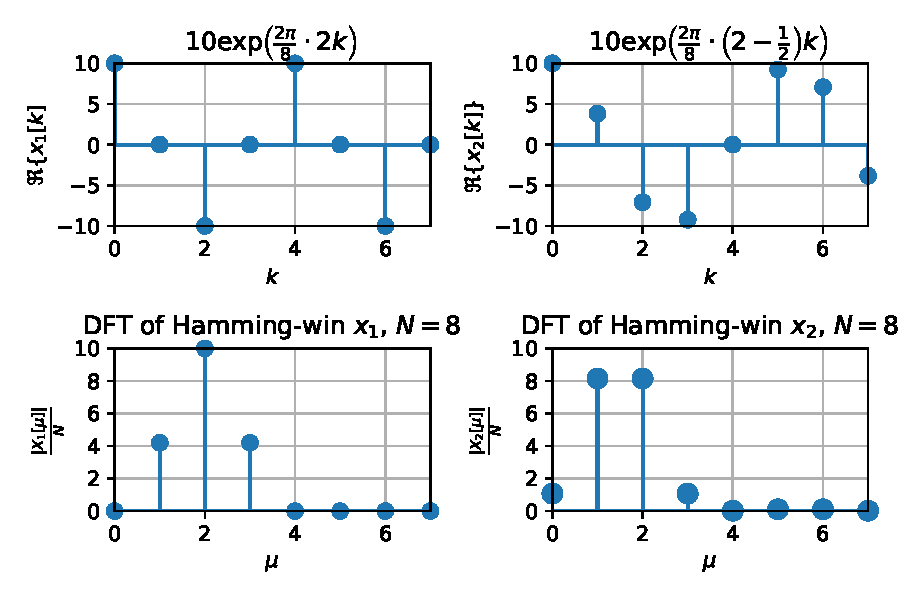
\includegraphics[width=6in, height=4in]{graphics/DFTbestworstcase_HammWin.pdf}
		\caption{Hamming windowing for $N=8$, best case ($\mu=2$),
		worst case ($\mu=2-\frac{1}{2}$).}
		\label{DFTbestworstcase_HammWin}
\end{figure}

%------------------------------------------------------------------------------
\cleardoublepage
\section{Exercises}

%------------------------------------------------------------------------------
\subsection*{Exercise 1: \texttt{dft}/\texttt{idft} Implementation}
\addcontentsline{toc}{subsection}{Exercise 1: \texttt{dft()}/\texttt{idft()} function}
Write Matlab/Python functions \texttt{X = my\_dft(x)} and \texttt{x = my\_idft(X)}
that calculate the DFT pair in eq.~\eqref{eq:DFT} and \eqref{eq:IDFT}
without using the pre-built functions \texttt{fft()} and \texttt{ifft()}.
%
Check validity and performance against the built-in functions (try large $N$).
%
We might consider the matrix operation approach rather than a for-loop
implementation.

\begin{Loesung}
\textbf{Solution:}
Jupyter Notebook: \texttt{dft\_windowing\_tutorial\_exercises.ipynb}
\\Matlab: \texttt{UE1\_Exercise1\_Test\_dft\_idft\_functions.m}
together with \texttt{my\_dft.m}, \texttt{my\_idft.m}
\end{Loesung}



% ---------------------------------------------------------------------------------
\subsection*{Exercise 2: IDFT as Analytic Calculus / as Linear Combination}
\addcontentsline{toc}{subsection}{Exercise 2: IDFT}
The discrete-time signal $x[k]$
\begin{equation}
x[k]=-2\cdot\sin\left(\frac{2\pi}{4}k\right)+3\cdot\cos\left(\frac{2\pi}{4}\cdot2k\right)+1
\hspace{5mm}\text{for}\,\,0\leq k\leq3
\end{equation}
with $k\in\mathbb{Z}$ is given.
\begin{enumerate}[label=\alph*)]
	\item Calculate the resulting values of $x[k]$ for $0\leq k\leq3$.
%
	\item Show analytically that the given values of $X[\mu]$, $\mu\in\mathbb{Z}$:
	\begin{equation}
	X[\mu=0]=4, \hspace{5mm} X[\mu=1]=4\im, \hspace{5mm} X[\mu=2]=12,
	\end{equation}
	are the DFT coefficients of $x[k]$ stemming from
	\begin{equation}
	X[\mu]=\sum_{k=0}^{N-1}x[k]\cdot\e^{-\im\frac{2\pi}{N}k\mu}
	\end{equation}
	with $N=4$.
%
	The following procedure is suggested: Setup the spectral
	coefficients $X[\mu]$ in the form
	\begin{equation}
	X[\mu]=A[\mu]\cdot\e^{\im\phi[\mu]}
	\end{equation}
	and specify the missing value $X[\mu=3]$ so that the IDFT results in
	$x[k]\in\mathbb{R}$.
%
	Then calculate the IDFT as
	\begin{equation}
	x[k]=\frac{1}{N}\sum_{\mu=0}^{N-1}X[\mu]\cdot\e^{\im\frac{2\pi}{N}k\mu}
	\end{equation}
	showing that this corresponds to the given signal $x[k]$.
%
	\item Plot the real and imaginary part as well as the magnitude and the phase
	of $X[\mu]$ over $\mu$.
%
	\item
  Remove the DC component in the DFT spectrum $X[\mu]$ and from that synthesise
  the signal $x_r[k]$ via IDFT.
  Check that the synthesised signal corresponds to
  \begin{equation}
  x_r[k]=-2\cdot\sin\left(\frac{2\pi}{4}k\right)+3\cdot\cos\left(\frac{2\pi}{4}\cdot2k\right)
  \hspace{5mm}\text{for}\,\,0\leq k\leq3
  \end{equation}
  by help of a linear combination using the Fourier matrix.
%
	\item A DFT-based audio analyser shall exhibit a frequency resolution of
	$\Delta f=0.5$~Hz for a sampling frequency $f_s=44100$~Hz using a rectangular
	window.
%
	Determine the minimum required DFT length $N$ when only lengths $N=2^M$
	($M\in\mathbb{N}$) are allowed.
%
	What is the resulting frequency resolution then?

\end{enumerate}

\begin{Loesung}
\textbf{Solution:}

Jupyter Notebook: \texttt{dft\_windowing\_tutorial\_exercises.ipynb}
\begin{enumerate}[label=\alph*)]
	\item \begin{align}
	x[0]&=-2\cdot\sin\left(2\pi\frac{1}{4}\cdot0\right)+3\cdot\cos\left(2\pi\frac{2}{4}\cdot0\right)+1=3+1=4\nonumber\\
	x[1]&=-2\cdot\sin\left(2\pi\frac{1}{4}\cdot1\right)+3\cdot\cos\left(2\pi\frac{2}{4}\cdot1\right)+1=-2-3+1=-4\nonumber\\
	x[2]&=-2\cdot\sin\left(2\pi\frac{1}{4}\cdot2\right)+3\cdot\cos\left(2\pi\frac{2}{4}\cdot2\right)+1=3+1=4\nonumber\\
	x[3]&=-2\cdot\sin\left(2\pi\frac{1}{4}\cdot3\right)+3\cdot\cos\left(2\pi\frac{2}{4}\cdot3\right)+1=2-3+1=0\nonumber
	\end{align}
	\item \begin{align}
	X[\mu=0]&=4=4\cdot\e^{\im\cdot0}\nonumber\\
	X[\mu=1]&=4\im=4\cdot\e^{\im\frac{\pi}{2}}\nonumber\\
	X[\mu=2]&=12=12\cdot\e^{\im\cdot0}\nonumber
	\end{align}
	For $x[k]\in\mathbb{R}$ the symmetry $X[1]^*=X[3]$ holds, thus
	\begin{align}
	X[\mu=3]=-4\im=4\cdot\e^{-\im\cdot\frac{\pi}{2}}.\nonumber
	\end{align}
	The IDFT is given as
	\begin{align}
	x[k]&=\frac{1}{N}\sum_{\mu=0}^{N-1}X[\mu]\cdot\e^{\im\frac{2\pi}{N}k\mu}\nonumber\\
	&=\frac{1}{4}\sum_{\mu=0}^{3}X[\mu]\cdot\e^{\im\frac{\pi}{2}k\mu}.\nonumber
	\end{align}
	With the spectral coefficients in the form $X[\mu]=A[\mu]\cdot\e^{\im\phi[\mu]}$ this simplifies to
	\begin{align}
  x[k]&=\frac{1}{4}(4\cdot\e^{\im\cdot0}\cdot\e^{\im\frac{\pi}{2}k\cdot0}+4\cdot\e^{\im\cdot\frac{\pi}{2}}\cdot\e^{\im\frac{\pi}{2}k\cdot1}+12\cdot\e^{\im\cdot0}\cdot\e^{\im\frac{\pi}{2}k\cdot2}+4\cdot\e^{-\im\cdot\frac{\pi}{2}}\cdot\e^{\im\frac{\pi}{2}k\cdot3})\nonumber\\
	&=1+\e^{\im\frac{\pi}{2}}\cdot\e^{\im\frac{\pi}{2}k}+3\cdot\e^{\im\pi k}+\e^{-\im\frac{\pi}{2}}\cdot\e^{\im\frac{3\pi}{2}k}\nonumber\\
	&=1+\e^{\im\frac{\pi}{2}}\cdot\e^{\im\frac{\pi}{2}k}+3\cdot\left(\cos(\pi k)+\underbrace{\im\cdot\sin(\pi k)}_{=0\,\,\mathrm{if}\,\,k\in\mathbb{Z}}\right)-\e^{\im\frac{\pi}{2}}\cdot\e^{-\im\frac{\pi}{2}k}\nonumber\\
	&=1+3\cdot\cos(\pi k)+\underbrace{\e^{\im\frac{\pi}{2}}}_{=\im}\cdot\left(\e^{\im\frac{\pi}{2}k}-\e^{-\im\frac{\pi}{2}k}\right).\nonumber
	\end{align}
 With Euler's identity
	\begin{equation}
	2\im\cdot\sin(x)=\e^{\im x}-\e^{-\im x}\nonumber
	\end{equation}
	we get
	\begin{align}
	x[k]&=1+3\cdot\cos(\pi k)+\im\cdot2\im\cdot\sin\left(\frac{\pi}{2}k\right)\nonumber\\
	&=1+3\cdot\cos(\pi k)-2\cdot\sin\left(\frac{\pi}{2}k\right)\nonumber
	\end{align}
	which finally results as expected
	\begin{equation}
	x[k]=1+3\cdot\cos\left(\frac{2\pi}{4}\cdot2k\right)-2\cdot\sin\left(\frac{2\pi}{4}k\right).\nonumber
	\end{equation}
	\item \text{}
	\begin{center}%
		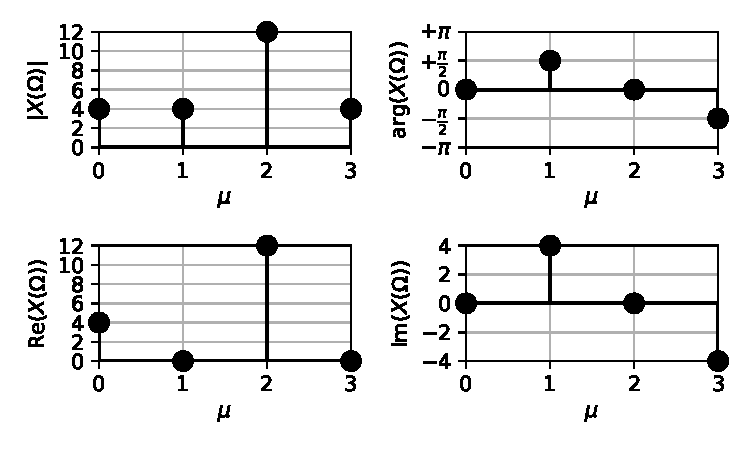
\includegraphics[width=5in, height=3in]{graphics/UE1_Exercise2_IDFT.pdf}%
		\captionof{figure}{DFT of $x[k]$ for exercise 2 c).}%
  \end{center}%
	\item
  Recall that the IDFT is given as $\bm x_k = \frac{1}{N} \bm W \bm x_\mu$ with
  the vectors
  \begin{align}
  \text{discrete-time signal: }
  \bm{x}_k =
  \begin{bmatrix}
  x[k=0]\\
  x[k=1]\\
  x[k=2]\\
  x[k=3]\\
  \vdots\\
  x[k=N-1]\\
  \end{bmatrix}\qquad
  \text{DFT spectrum: }
  \bm{x}_\mu =
  \begin{bmatrix}
  X[\mu=0]\\
  X[\mu=1]\\
  X[\mu=2]\\
  X[\mu=3]\\
  \vdots\\
  X[\mu=N-1]\\
  \end{bmatrix}.
  \end{align}
  and the Fourier matrix $\bm W$.

  The samples of the DC-free signal $x_r[k]$ set up as a column vector are
 \begin{align}
 \mathbf{xr}_{k} =
 \begin{bmatrix}
 x_r[k=0]=3\\x_r[k=1]=-5\\x_r[k=2]=3\\x_r[k=0]=-1
 \end{bmatrix}
 \end{align}
  just by subtracting the DC amount 1 from $x[k]$.
  %
  Let us check the IDFT by matrix multiplication.
	%
	We build the $4\times 4$ Fourier matrix (by element-wise operation)
	\begin{equation}
	\mathbf{W} = \mathrm{e}^{+\mathrm{j}\frac{2\pi}{4} \mathbf{K}}
	\end{equation}
	from the twiddle factor
	\begin{equation}
	W_{N=4} = \mathrm{e}^{+\mathrm{j}\frac{2\pi}{4}}
	\end{equation}
	and from matrix (this is an outer product)
	\begin{equation}
	\mathbf{K} =
	\begin{bmatrix}
	0\\
	1\\
	2\\
	3
	\end{bmatrix}
	\cdot
	\begin{bmatrix}
	0 & 1 & 2 & 3
	\end{bmatrix}
  =
	\begin{bmatrix}
	0 & 0 & 0 & 0\\
	0 & 1 & 2 & 3\\
	0 & 2 & 4 & 6\\
	0 & 3 & 6 & 9
	\end{bmatrix}
	\end{equation}
	containing all possible products $k\,\mu$ in a suitable arrangement.
	%
	We get
	\begin{align}
	\mathbf{W} = \begin{bmatrix}
	1 & 1 & 1 & 1\\
	1 & +\mathrm{j} & -1 & -\mathrm{j}\\
	1 & -1 & 1 & -1\\
	1 & -\mathrm{j} & -1 & +\mathrm{j}
	\end{bmatrix}
  \end{align}
  The columns are the DFT signals
  \begin{align}
	\mathbf{w}_1 = \begin{bmatrix}1\\1\\1\\1\end{bmatrix},
	\mathbf{w}_2 = \begin{bmatrix}1\\+\im\\-1\\-\im\end{bmatrix},
	\mathbf{w}_3 = \begin{bmatrix}1\\-1\\1\\-1\end{bmatrix},
	\mathbf{w}_4 = \begin{bmatrix}1\\-\im\\-1\\+\im\end{bmatrix}.
	\end{align}
  to be used for the linear combination
	\begin{equation}
	\mathbf{xr}_k =
  \frac{X[\mu=0]}{4} \, \mathbf{w}_1
	+ \frac{X[\mu=1]}{4} \,\mathbf{w}_2
	+ \frac{X[\mu=2]}{4} \,\mathbf{w}_3
	+ \frac{X[\mu=3]}{4} \,\mathbf{w}_4.
	\end{equation}
  using the DFT coefficients from task b).

	As $X[\mu=0]$ shall be made zero by intention we are left with the
  linear combination
	\begin{equation}
  \mathbf{xr}_k=
  \frac{0}{4}\cdot\begin{bmatrix}1\\1\\1\\1\end{bmatrix}+
	\frac{+4\im}{4}\cdot\begin{bmatrix}1\\+\im\\-1\\-\im\end{bmatrix}+
	\frac{12}{4}\cdot\begin{bmatrix}1\\-1\\1\\-1\end{bmatrix}+
	\frac{-4\im}{4}\cdot\begin{bmatrix}1\\-\im\\-1\\+\im\end{bmatrix}
  =
  \begin{bmatrix}
  3\\-5\\3\\-1
  \end{bmatrix}
	\end{equation}
  which gives the desired result.
%
  \item \begin{align}
  \Delta f=\frac{f_s}{N}=\frac{f_s}{2^M}&\stackrel{!}{=}0.5\,\text{Hz}\nonumber\\
  M&=\left\lceil\log_{2}\left(\frac{f_s}{\Delta f}\right)\right\rceil_{\in\mathbb{N}}\nonumber\\
  &=\left\lceil\log_{2}\left(\frac{44100\,\text{Hz}}{0.5\,\text{Hz}}\right)\right\rceil_{\in\mathbb{N}}\nonumber\\
  &=\left\lceil16.4285...\right\rceil_{\in\mathbb{N}}\nonumber\\
  &=17\nonumber\\
  \Rightarrow\hspace{5mm} N&=2^M=2^{17}=131072\nonumber
  \end{align}
  The resulting frequency resolution is thus
  \begin{equation}
  \Delta f=\frac{f_s}{N}=\frac{44100\,\text{Hz}}{131072}\approx0.3365\,\text{Hz}.\nonumber
  \end{equation}
%
\end{enumerate}
\end{Loesung}



%------------------------------------------------------------------------------
\subsection*{Exercise 3: DFT Analysis Using a Rectangular Window / DTFT Interpolation}
\addcontentsline{toc}{subsection}{Exercise 3: DFT Analysis Using a Rectangular Window}
A sine signal $x[k]=\cos(\Omega k)$ with $\Omega=2\cdot\frac{2\pi}{N}$, $N=8$,
$0\leq k \leq N-1$ is to be analysed with the DFT eq.~\eqref{eq:DFT} assuming a
sampling frequency of $f_s=48$~kHz.
%
\begin{enumerate}[label=\alph*)]
	\item Calculate the spectrum $X[\mu]$ of $x[k]$ and visualise the real and
	imaginary part as well as the magnitude and the phase of $X[\mu]$ over
	$0\leq\mu\leq N-1$.
%
	\item Check the expected symmetries.
%
	\item Implement the interpolation of eq.~\eqref{eq:DTFT_Interpolation_psinc}
	and visualise this over $\mu$, $\Omega$ as well as $f$ as a magnitude
	spectrum together with $|X[\mu]|$.
%
	\item Repeat the steps a) to c) for $N=9$. What is different?
%
	\item Repeat the steps a) to d) for $\Omega=2.5\cdot\frac{2\pi}{N}$.
	What is different now?
\end{enumerate}

\begin{Loesung}
\textbf{Solution:}

Jupyter Notebook: \texttt{dft\_windowing\_tutorial\_exercises.ipynb}

Matlab: \texttt{UE1\_Exercise3\_DFT\_analysis.m}
together with \texttt{interpolate\_DFT.m}
\end{Loesung}



% ---------------------------------------------------------------------------------
\subsection*{Exercise 4: DFT / DTFT of an Impulse Response}
\addcontentsline{toc}{subsection}{Exercise 4: DFT of an impulse response}
The finite length impulse response (FIR filter) $h[k]$ of an LTI system is given
as
%
\begin{equation}
h[k]=\frac{1}{8}\cdot\left(11\cdot\delta[k]-5\cdot\delta[k-1]+7\cdot\delta[k-2]-9\cdot\delta[k-3]\right)
\end{equation}
%
The DFT and DTFT spectrum correspond to the transfer function of the system.

\begin{enumerate}[label=\alph*)]
	\item Calculate the DFT analytically
%
	\begin{equation}
	H[\mu]=\sum_{k=0}^{N-1}h[k]\cdot\e^{-\im\frac{2\pi}{N}k\mu}
	\end{equation}
	for $N=4$ and $0\leq k\leq N-1$.
%
	\item Calculate the magnitude $|H[\mu]|$ and the phase response $\arg(H[\mu])$
	for $0\leq\mu\leq 3$. State the magnitude as level in dB and the phase in
	degrees.
%
	\item The frequency resolution is assumed to be $\Delta f=500\,\text{Hz}$.
	Sketch the DFT line spectrum and the interpolated DTFT spectrum of the
	magnitude $|H[\mu]|$ in dB and the phase $\arg(H[\mu])$ in degrees over the
	frequency axis from $0\,\text{Hz}\leq f\leq4000\,\text{Hz}$.
	Estimate the sampling frequency $f_s$ from the known parameters and information.
	What filter characteristic is realised with this impulse response?
\end{enumerate}

\begin{Loesung}
\textbf{Solution:}
\begin{enumerate}[label=\alph*)]
	\item
  If we set up the FIR $h[k]$ and the DFT spectrum $H[\mu]$ as vectors
  \begin{equation}
  \mathbf{h}_k =
  \begin{bmatrix}
  h[k=0]\\
  h[k=1]\\
  h[k=2]\\
  h[k=3]\\
  \end{bmatrix}
  =
  \frac{1}{8}
  \begin{bmatrix}
  11\\
  -5\\
  7\\
  -9\\
  \end{bmatrix}
  \qquad
  \mathbf{h}_\mu =
  \begin{bmatrix}
  H[\mu=0]\\
  H[\mu=1]\\
  H[\mu=2]\\
  H[\mu=3]\\
  \end{bmatrix}
  \end{equation}
  the DFT can be calculated with matrix multiplication,
  cf. Section \ref{Ch:DFTasMatrixOperation},
  \begin{equation}
  \mathbf{h}_\mu = \mathbf{W}^* \mathbf{h}_k
  \end{equation}
  using again the $4 \times 4$ Fourier matrix (see exercise 2)
  \begin{align}
  \mathbf{W} = \begin{bmatrix}
  1 & 1 & 1 & 1\\
  1 & +\mathrm{j} & -1 & -\mathrm{j}\\
  1 & -1 & 1 & -1\\
  1 & -\mathrm{j} & -1 & +\mathrm{j}
  \end{bmatrix}
  \end{align}
  The columns of $\bm W$ are the DFT eigensignals
  \begin{align}
  \mathbf{w}_\text{column 1} = \begin{bmatrix}1\\1\\1\\1\end{bmatrix},
  \mathbf{w}_\text{column 2} = \begin{bmatrix}1\\+\im\\-1\\-\im\end{bmatrix},
  \mathbf{w}_\text{column 3} = \begin{bmatrix}1\\-1\\1\\-1\end{bmatrix},
  \mathbf{w}_\text{column 4} = \begin{bmatrix}1\\-\im\\-1\\+\im\end{bmatrix}.
  \end{align}
  The DFT is the signal analysis stage, i.e. correlation of the input signal with
  DFT eigensignals. This is realised by the (complex) inner product of the two vectors.
  Thus, the inner products $H[\mu] = \mathbf{w}_{\text{column } (\mu+1)}^\text{H} \mathbf{h}_k$
  requires complex conjugates
  \begin{align}
  &\mathbf{w}_\text{column 1}^\text{H} = \begin{bmatrix}1, 1, 1, 1\end{bmatrix}\nonumber\\
  &\mathbf{w}_\text{column 2}^\text{H} = \begin{bmatrix}1,-\im,-1,+\im\end{bmatrix}\nonumber\\
  &\mathbf{w}_\text{column 3}^\text{H} = \begin{bmatrix}1,-1,1,-1\end{bmatrix}\nonumber\\
  &\mathbf{w}_\text{column 4}^\text{H} = \begin{bmatrix}1,+\im,-1,-\im\end{bmatrix}.
  \end{align}
  Calculated for all $\mu$ this yields the DFT spectrum
  \begin{align}
  H[\mu=0]&=\mathbf{w}_{\text{column 1}}^\text{H} \mathbf{h}_k = \left(1\cdot\frac{11}{8}\right)+\left(1\cdot\frac{-5}{8}\right)+\left(1\cdot\frac{7}{8}\right)+\left(1\cdot\frac{-9}{8}\right)=\frac{4}{8}=\frac{1}{2}\nonumber\\
  H[\mu=1]&=\mathbf{w}_{\text{column 2}}^\text{H} \mathbf{h}_k = \left(1\cdot\frac{11}{8}\right)+\left((-\im)\cdot\frac{-5}{8}\right)+\left((-1)\cdot\frac{7}{8}\right)+\left(\im\cdot\frac{-9}{8}\right)=\frac{4}{8}-\im\frac{4}{8}=\frac{1}{2}-\im\frac{1}{2}\nonumber\\
  H[\mu=2]&=\mathbf{w}_{\text{column 3}}^\text{H} \mathbf{h}_k= \left(1\cdot\frac{11}{8}\right)+\left((-1)\cdot\frac{-5}{8}\right)+\left(1\cdot\frac{7}{8}\right)+\left((-1)\cdot\frac{-9}{8}\right)=\frac{32}{8}=4\nonumber\\
  H[\mu=3]&=\mathbf{w}_{\text{column 4}}^\text{H} \mathbf{h}_k= \left(1\cdot\frac{11}{8}\right)+\left(\im\cdot\frac{-5}{8}\right)+\left((-1)\cdot\frac{7}{8}\right)+\left((-\im)\cdot\frac{-9}{8}\right)=\frac{4}{8}+\im\frac{4}{8}=\frac{1}{2}+\im\frac{1}{2}\nonumber
  \end{align}

	\item \begin{align}
	|H[0]|&=\frac{1}{2} \hspace{5mm}\longrightarrow\hspace{5mm} 20\log_{10}\left(\frac{1}{2}\right)=-6.02\,\text{dB}\nonumber\\
	|H[1]|&=\sqrt{\frac{1}{2^2}+\frac{1}{2^2}}=\frac{1}{\sqrt{2}} \hspace{5mm}\longrightarrow\hspace{5mm} 20\log_{10}\left(\frac{1}{\sqrt{2}}\right)=-3.01\,\text{dB}\nonumber\\
	|H[2]|&=4 \hspace{5mm}\longrightarrow\hspace{5mm} 20\log_{10}(4)=12.04\,\text{dB}\nonumber\\
	|H[3]|&=\sqrt{\frac{1}{2^2}+\frac{1}{2^2}}=\frac{1}{\sqrt{2}} \hspace{5mm}\longrightarrow\hspace{5mm} 20\log_{10}\left(\frac{1}{\sqrt{2}}\right)=-3.01\,\text{dB}\nonumber\\
	\arg(H[0])&=0\nonumber\\
	\arg(H[1])&=\arctan\left(\frac{-\frac{1}{2}}{\frac{1}{2}}\right)=-0.7854\,\hat{=}\,-45^{\circ}\nonumber\\
	\arg(H[2])&=0\nonumber\\
	\arg(H[3])&=\arctan\left(\frac{\frac{1}{2}}{\frac{1}{2}}\right)=0.7854\,\hat{=}\,45^{\circ}\nonumber
	\end{align}
	\item \text{}
	\begin{center}%
		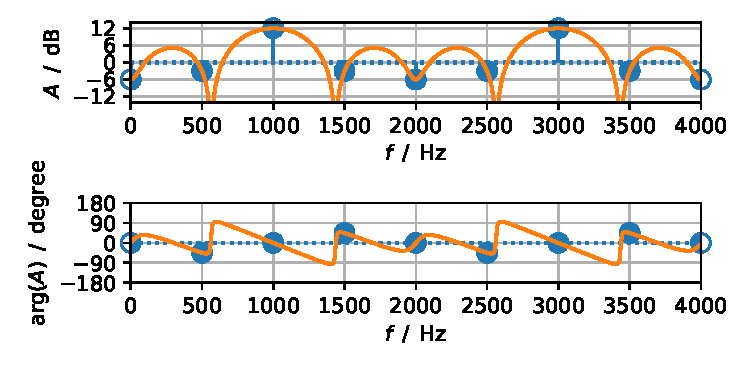
\includegraphics[width=5in, height=2.5in]{graphics/UE1_Exercise4_Spectrum.pdf}%
		\captionof{figure}{DFT (blue dots) and DTFT (red line) spectrum for $h[k]$}%
	\end{center}%
	\underline{sampling frequency:} $\Delta f=\frac{f_s}{N}\,\,\Leftrightarrow\,\,f_s=\Delta f\cdot N=500\,\text{Hz}\cdot4=2000\,\text{Hz}$\\\\
	\underline{filter characteristic:} highpass filter, -3~dB corner frequency at
	about 790~Hz, relative sidelobe level about -7~dB, notch at about 560~Hz,
	12~dB gain at $\frac{f_s}{2}$
\end{enumerate}
\end{Loesung}



% ---------------------------------------------------------------------------------
\subsection*{Exercise 5: DFT Parameterisation}
\addcontentsline{toc}{subsection}{Exercise 5: DFT parameterisation}
A composite signal
$x[k]=A_1\cdot\e^{\im(\Omega_1 k+\phi_1)}+A_2\cdot\e^{\im(\Omega_2 k+\phi_2)}$
with the known frequencies $\Omega_1=\frac{1}{30}\pi$ and $\Omega_2=\frac{1}{4}\pi$
but unknown amplitude and phase relation is given.
%
\begin{enumerate}[label=\alph*)]
	\item What DFT length $N$ must be set up so that the exact amplitude and
	phase values for both frequencies $\Omega_1$ and $\Omega_2$ can be determined
	for a rectangularly windowed signal (i.e. no leakage occurs)?
%
	\item In which bins are the frequencies $\Omega_1$ and $\Omega_2$ then found?
%
	\item What amplitude deviation occurs when analysing the signal
	$x[k]=\e^{\im\Omega_3k}$ with $\Omega_3=\frac{30.5}{60}\pi$?
\end{enumerate}

\begin{Loesung}
\textbf{Solution:}
\begin{enumerate}[label=\alph*)]
	\item DFT eigenfrequencies: $\Omega_\text{DFT}=\frac{2\pi}{N}\mu$\\\\
	$\Omega_1$ and $\Omega_2$ must be DFT eigenfrequencies (recall $\mu\in\mathbb{Z}$):
%
	\begin{align}
	\Omega_1&=\frac{\pi}{30}=\frac{2\pi}{N}\mu \hspace{5mm}\Leftrightarrow\hspace{5mm} N=60\cdot\mu\nonumber\\
	\Omega_2&=\frac{\pi}{4}=\frac{2\pi}{N}\mu \hspace{5mm}\Leftrightarrow\hspace{5mm} N=8\cdot\mu\nonumber
	\end{align}
%
	Both conditions together can be fulfilled when using $N=120$ (or multiples thereof).
%
	\item \begin{align}
	\mu_1&=\Omega_1\cdot\frac{N}{2\pi}=\frac{\pi}{30}\cdot\frac{120}{2\pi}=2, \hspace{5mm}\text{i.e. the 3rd bin / column of } \bm W\nonumber\\
	\mu_2&=\Omega_2\cdot\frac{N}{2\pi}=\frac{\pi}{4}\cdot\frac{120}{2\pi}=15, \hspace{5mm}\text{i.e. the 16th bin / column of } \bm W\nonumber
	\end{align}
%
	\item The discrete angular frequency $\Omega_3=\frac{30.5}{60}\pi$ can be
	expressed in terms of multiples of the first DFT eigenfrequency
	$\frac{2\pi}{N}$ as
%
	\begin{equation}
	\Omega_3=n\cdot\frac{2\pi}{N} \hspace{5mm}\leftrightarrow\hspace{5mm} n=\Omega_3\cdot\frac{N}{2\pi}=\frac{30.5}{60}\pi\cdot\frac{120}{2\pi}=30.5\nonumber
	\end{equation}
%
	so that
%
	\begin{equation}
	\Omega_3=30.5\cdot\frac{2\pi}{N}.\nonumber
	\end{equation}
%
	The frequency $\Omega_3$ is not a DFT eigenfrequency as it is not an integer
	multiple of the first DFT eigenfrequency, but is located in the middle between
	bins 31 and 32 (for $\mu=30$ and $\mu=31$ counting from $\mu=0$).
%
	The neighbouring bins are the bins that can give the best information about
	the amplitude of the true signal.
%
	The spectral values at the neighbouring bins can be calculated by the DFT of
	a complex exponential (see formularies)
%
	\begin{equation}
	\e^{\im\Omega_3 k} \hspace{5mm}\laplace\hspace{5mm} \e^{\im\frac{\left(\Omega_3-\frac{2\pi}{N}\mu\right)(N-1)}{2}}\cdot\frac{\sin\left(N\frac{\Omega_3-\frac{2\pi}{N}\mu}{2}\right)}{\sin\left(\frac{\Omega_3-\mu\frac{2\pi}{N}}{2}\right)}.\nonumber
	\end{equation}
%
	At $\mu=30$, the amplitude is
%
	\begin{align}
	|X[\mu=30]|&=\left|\e^{\im\frac{\left(\Omega_3-\frac{2\pi}{N}\mu\right)(N-1)}{2}}\cdot\frac{\sin\left(N\frac{\Omega_3-\frac{2\pi}{N}\mu}{2}\right)}{\sin\left(\frac{\Omega_3-\frac{2\pi}{N}\mu}{2}\right)}\right|\nonumber\\
	&=\frac{\sin\left(N\frac{\Omega_3-\frac{2\pi}{N}\mu}{2}\right)}{\sin\left(\frac{\Omega_3-\frac{2\pi}{N}\mu}{2}\right)}\nonumber\\
	&=\frac{\sin\left(N\frac{30.5\cdot\frac{2\pi}{N}-30\cdot\frac{2\pi}{N}}{2}\right)}{\sin\left(\frac{30.5\cdot\frac{2\pi}{N}-30\cdot\frac{2\pi}{N}}{2}\right)}\nonumber\\
	&=\frac{\sin\left(N\frac{\frac{1}{2}\cdot\frac{2\pi}{N}}{2}\right)}{\sin\left(\frac{\frac{1}{2}\cdot\frac{2\pi}{N}}{2}\right)}\nonumber\\
	&=\frac{\sin\left(\frac{\pi}{2}\right)}{\sin\left(\frac{\pi}{2N}\right)}\nonumber\\
	&=\frac{1}{\sin\left(\frac{\pi}{240}\right)}\nonumber\\
	&\approx76.3966.\nonumber
	\end{align}
%
	At $\mu=31$, the amplitude is
%
	\begin{align}
	|X[\mu=31]|&=\frac{\sin\left(N\frac{30.5\cdot\frac{2\pi}{N}-31\cdot\frac{2\pi}{N}}{2}\right)}{\sin\left(\frac{30.5\cdot\frac{2\pi}{N}-31\cdot\frac{2\pi}{N}}{2}\right)}\nonumber\\
	&=\frac{\sin\left(-\frac{\pi}{2}\right)}{\sin\left(-\frac{\pi}{2N}\right)}\nonumber\\
	&\approx76.3966.\nonumber
	\end{align}
%
	If the frequency of the complex exponential had been exactly at a DFT
	eigenfrequency, e.g. at $\mu=31$, the DFT spectrum would have contained the
	true amplitude of the signal.
	The rule of L'Hospital is needed to to calculate this amplitude value:
%
	\begin{align}
	&\lim_{\Omega_3\to31\cdot\frac{2\pi}{N}}\frac{\sin\left(N\frac{\Omega_3-\frac{2\pi}{N}31}{2}\right)}{\sin\left(\frac{\Omega_3-\frac{2\pi}{N}31}{2}\right)}\nonumber\\
	=&\lim_{\Omega_3\to31\cdot\frac{2\pi}{N}}\frac{\cos\left(N\frac{\Omega_3-\frac{2\pi}{N}31}{2}\right)\cdot\frac{N}{2}}{\cos\left(\frac{\Omega_3-\frac{2\pi}{N}31}{2}\right)\cdot\frac{1}{2}}\nonumber\\
	=&\frac{\cos0}{\cos0}\cdot N\nonumber\\
	=&N\nonumber\\
	=&120\nonumber.
	\end{align}
%
	The error is thus
	\begin{equation}
	20\cdot\log_{10}\left(\frac{76.3966}{120}\right)=-3.9221\,\text{dB},\nonumber
	\end{equation}
	i.e. the magnitude is underestimated.
	The case when the signal frequency lies exactly in middle between two DFT
	eigenfrequencies is the worst case scenario, in \cite{Harris1978}
	termed "worst case process loss".
\end{enumerate}
\end{Loesung}

%------------------------------------------------------------------------------
%\bibliographystyle{Schultz_PHD}
%\bibliographystyle{IEEEtran}
\bibliography{literature}
\end{document}
